%%%%%%%%%%%%%%%%%%%%%%%%%%%%%%%%%%%%%%%%%
% OIST Thesis (Proposal)
% LaTeX Template
% Version 0.3 (2025/08/26)
%
% This version covers the thesis proposal, the electronic thesis, and the
% printed and bound thesis. For information on how to choose these, see
% the guide in the default chapters, which can also be found in the
% Github repository:
% https://github.com/oist/LaTeX-template-phd-thesis
%
% Authors:
% Jeremie Gillet
% Jack Featherstone
%
%%%%%%%%%%%%%%%%%%%%%%%%%%%%%%%%%%%%%%%%%

%----------------------------------------------------------------------------------------
%	BINDING STYLE (pick the style you want)
%----------------------------------------------------------------------------------------

\RequirePackage{etoolbox}
\newtoggle{bind}

% The thesis proposal and early drafts of the thesis are not going
% to be printed as a book, so you want a "one-sided" page style with even margins.
% To set defaults for this, use the following line.
\togglefalse{bind}

% But for the final draft of the thesis, you probably want to print a copy
% and bind it, so you need alternating headers/footers on pages, different
% margins, etc. To set defaults for this, use the following line.
%\toggletrue{bind}

%----------------------------------------------------------------------------------------
%	PACKAGES AND OTHER DOCUMENT CONFIGURATIONS
%----------------------------------------------------------------------------------------

% Choose either a two-sided or one-sided book, depending on the value of
% `bind`.
\iftoggle{bind}{
    % 12 pt font for main body text, and a two-sided book style (so margins
    % alternate on even and off pages) 
    \documentclass[12pt, twoside]{book}
    % A4 paper size, inner margin is 3cm, all others are 2.5cm
    \usepackage[a4paper, includehead, headheight=0.6cm, inner=3cm, outer=2.5cm, top=2.5 cm, bottom=2.5cm]{geometry}  % Changing size of document

}{ % Else
    % 12 pt font for main body text, and a one-sided book style (so margins
    % don't alternate every other page) 
    \documentclass[12pt, oneside]{book}
    % A4 paper size, left margin is 3cm, all others are 2.5cm
    \usepackage[a4paper, includehead, headheight=0.6cm, left=3cm, right=2.5cm, top=2.5 cm, bottom=2.5cm]{geometry}  % Changing size of document

}

\usepackage[english]{babel} % The document is in English
\usepackage[utf8]{inputenc} % UTF8 encoding
\usepackage[T1]{fontenc} % Font encoding

\usepackage{graphicx} % For including images
\graphicspath{{./Images/}} % Specifies the directory where pictures are stored

\usepackage{longtable} % tables that can span several pages
\usepackage[bf, font=footnotesize]{caption} % caption: FIG in bold and 10pt (footnotesize) captions
\usepackage{fancyhdr} % For the headers
% This is imported below so we can have a conditional that controls
% single or 1.5
%\usepackage[onehalfspacing]{setspace} % For 1.5 spacing

%----------------------------------------------------------------------------------------
%	HEADERS AND FOOTERS
%----------------------------------------------------------------------------------------
% Our header and footer setup is different depending on whether we are
% looking to bind our final result or not.

\iftoggle{bind}{
    \newcommand{\numberedchapter}{ % Preparation for numbered chapters
        \cleardoublepage % To make sure the previous headers are passed

        % For binding, we have the page number on the outside
        \fancyhead[RO,LE]{\thepage}

        % The chapter on the even page right side, and the section on
        % the odd page left side.
        \fancyhead[RE]{{\bfseries \leftmark}}
        \fancyhead[LO]{{\bfseries \rightmark}}
    }

    \newcommand{\unnumberedchapter}[1]{ % Preparation for unnumbered chapters 
        \cleardoublepage % To make sure the previous headers are passed
        \phantomsection % To make sure the table of content links to the right page
        \addcontentsline{toc}{chapter}{#1} % Also adds the chapter name to the Contents

        % For unnumbered chapters, we have the page number the same as
        % for numbered ones, on the outside
        \fancyhead[RO,LE]{\thepage}
    
        % Though we have to manually set the section name because it is
        % unnumbered
        \fancyhead[RE]{{\bfseries #1}} % Headers for left pages
        \fancyhead[LO]{} % Headers for right pages
    }

}{ % Else
    \newcommand{\numberedchapter}{ % Preparation for numbered chapters
            \cleardoublepage % To make sure the previous headers are passed

            % For non-binding, we have the page number always on the right
            \fancyhead[R]{\thepage}
            % And current section on the left
            \fancyhead[L]{{\bfseries \rightmark}}
    }

    \newcommand{\unnumberedchapter}[1]{ % Preparation for unnumbered chapters
            \cleardoublepage % To make sure the previous headers are passed
            \phantomsection % To make sure the table of content links to the right page
            \addcontentsline{toc}{chapter}{#1} % Also adds the chapter name to the Contents
            % For non-binding, we have the page number always on the right
            \fancyhead[R]{\thepage}
            % And current section on the left
            \fancyhead[L]{{\bfseries \rightmark}}
    }
}

% Note that there is another section below that sets the header behavior
% for the regular pages; we can't set it here because we first need
% the preamble to have no header.


%----------------------------------------------------------------------------------------
%	BACKGROUND PICTURE ON TITLE PAGE
%----------------------------------------------------------------------------------------
\usepackage{emptypage} % No headers on an empty page

\usepackage{tikz}
\usepackage{eso-pic} % For the background picture on the title page
\newcommand\BackgroundPic{%
\put(-250,-160){%
\parbox[b][\paperheight]{\paperwidth}{%
\vfill
\centering

\includegraphics[width=\paperwidth]{symbol.jpg}%
\vfill
}}}

%----------------------------------------------------------------------------------------
%	LINKS
%----------------------------------------------------------------------------------------

% Clickable links for references, but don't put a box around them.
\usepackage[hidelinks]{hyperref}

% If you want to add colors to links (not boxes, but the link text itself)
% you can uncomment these lines.
%\hypersetup{
%    colorlinks   = true, % Color links instead of boxes
%    urlcolor     = {blue!50!black}, % Dark blue color for external hyperlinks
%    linkcolor    = {blue!50!black}, % Dark blue color for internal links
%    citecolor    = {red!50!black} % Dark red color for citations
%}

%----------------------------------------------------------------------------------------
%	IMPORT FROM mydefinitions.tex
%----------------------------------------------------------------------------------------

% First we setup the various conditionals and their defaults that can be
% adjusted in mydefinitions

% Whether the document is a thesis or thesis proposal
\newtoggle{isthesis}
\togglefalse{isthesis}

% Whether to use single or 1.5 spacing
\newtoggle{singlespacing}
\togglefalse{singlespacing}

% This includes your name, supervisors, title, etc.
%----------------------------------------------------------------------------------------
%	VALUES FOR THE THESIS (PROPOSAL)
%----------------------------------------------------------------------------------------

\newcommand{\name}{Your name} % Author name
\newcommand{\thesistitle}{\LaTeX\ thesis (proposal) template} % Title of the thesis
\newcommand{\submissiondate}{August 2025} % Submission date "Month year"
\newcommand{\supervisor}{S.~Upervisor} % Supervisor name
\newcommand{\cosupervisor}{C.~O'Supervisor} % Co-Supervisor name, comment this line if there is none

%----------------------------------------------------------------------------------------
%	TYPE OF DOCUMENT
%----------------------------------------------------------------------------------------
% If this is a thesis proposal make sure the line below is commented.
% If this is a thesis, uncomment the line below.
\toggletrue{isthesis}

%----------------------------------------------------------------------------------------
%	BINDING STYLE (pick the style you want)
%----------------------------------------------------------------------------------------
% This option must be set at the top of the Thesis_proposal.tex file (because
% it affects the document class). Go there and choose whether the document
% should be set up for printing and binding, or as a digital copy.

%----------------------------------------------------------------------------------------
%	TEXT SPACING
%----------------------------------------------------------------------------------------
% Unless you are submitting the final version of your thesis, the formatting
% guidelines request you to use 1.5 spacing (the default option). To change to
% single spacing for the final version, uncomment the line below:
%\toggletrue{singlespacing}

%----------------------------------------------------------------------------------------
%	BIBLIOGRAPHY STYLE (pick the style you want)
%----------------------------------------------------------------------------------------

\usepackage[square, numbers, sort&compress]{natbib} % for bibliography - Square brackets, citing references with numbers, citations sorted by appearance in the text and compressed (as in [4-7])
%\usepackage[longnamesfirst,round]{natbib} % Natural Sciences bibliography

\bibliographystyle{Preamble/physics_bibstyle} % You may use a different style adapted to your field
%\bibliographystyle{unsrtnat} % You may use a different style adapted to your field


%----------------------------------------------------------------------------------------
%	YOUR PACKAGES (be careful of package interaction)
%----------------------------------------------------------------------------------------

\usepackage{amsthm,amsmath,amssymb,amsfonts,bbm}% Math symbols

% In case you need to use Japanese characters (eg. for references) but this
% only works with xelatex as your compiler.
%\usepackage{xeCJK}
%\setCJKmainfont{Noto Serif CJK JP}

%----------------------------------------------------------------------------------------
%	YOUR DEFINITIONS AND COMMANDS
%----------------------------------------------------------------------------------------

% New Commands
\newcommand{\bea}{\begin{eqnarray}} % Shortcut for equation arrays
\newcommand{\eea}{\end{eqnarray}}
\newcommand{\e}[1]{\times 10^{#1}}  % Powers of 10 notation

% Defining a theorem box for Criteria
\newtheorem{critere}{Criterion}
\newcommand{\crit}[2]{
\begin{center}  
\fbox{ \begin{minipage}[c]{0.9 \textwidth}
\begin{critere}
\textbf{\textup{ #1}} --- #2
\end{critere}
\end{minipage}  } \end{center}
}



\iftoggle{singlespacing}{

    \usepackage[singlespacing]{setspace} % For 1 spacing
}{ % Else

    \usepackage[onehalfspacing]{setspace} % For 1.5 spacing
}

% We also need to change the font size for tables to 10pt, so we
% define a wrapper environment
\usepackage{floatrow}
\DeclareFloatFont{footnotesize}{\footnotesize}% "scriptsize" is defined by floatrow, "tiny" not
\floatsetup[table]{font=footnotesize}

%----------------------------------------------------------------------------------------
%	TITLE PAGE
%----------------------------------------------------------------------------------------
\begin{document}

\pagestyle{empty} % No page numbers
\frontmatter % Use roman page numbering style (i, ii, iii, iv...) for the preamble pages

\begin{titlepage}
\AddToShipoutPicture*{\BackgroundPic}
\begin{center}
\vfill
{\large \scshape Okinawa Institute of Science and Technology\\Graduate University}\\[1.4cm]
\iftoggle{isthesis}{
    \vspace{-0.8cm}
    {\large Thesis submitted for the degree}\\[0.5cm]
    {\Large Doctor of Philosophy}\\[0.5cm]
}{ % Else
    {\Large PhD Thesis Proposal}\\[0.5cm]
}
\rule{\textwidth}{1.5pt}\\[0cm]
{\huge \bfseries \thesistitle \par \ }\\[-0.5cm]
\rule{\textwidth}{1.5pt}\\[2.5cm]
\hfill  by\\[1cm]
\hfill  {\large \bfseries\name}\\
\vfill
{\hfill \large Supervisor: \textbf{\supervisor}} \\ 
\ifx\cosupervisor\undefined\else{\hfill \large Co-Supervisor: \textbf{\cosupervisor}} \\ \fi
\vspace{1cm}
\hfill  \submissiondate
\end{center}
\end{titlepage}

%----------------------------------------------------------------------------------------
%	PREAMBLE PAGES (comment out unnecessary pages)
%----------------------------------------------------------------------------------------

% Header and footer settings

\pagestyle{fancy} % Changes the headers
\renewcommand{\chaptermark}[1]{ \markboth{#1}{}} % Getting the chapter name right
\renewcommand{\sectionmark}[1]{\markright{\thesection\; #1}} % Getting the section name right
\fancyhf{}% Clears header and footer

\unnumberedchapter{Declaration of Original and Sole Authorship} 
\chapter*{Declaration of Original and Sole Authorship} 

I, \name, declare that this thesis entitled \emph{\thesistitle} and the data presented in it are original and my own work. 


I confirm that:
\begin{itemize}
\item No part of this work has previously been submitted for a degree at this or any other university.
\item References to the work of others have been clearly acknowledged. Quotations from the work of others have been clearly indicated, and attributed to them.
\item In cases where others have contributed to part of this work, such contribution has been clearly acknowledged and distinguished from my own work.
\item None of this work has been previously published elsewhere, with the exception of the following: (provide list of publications or presentations, or delete this part).  (If the work of any co-authors appears in this thesis, authorization such as a release or signed waiver from all affected co-authors must be obtained prior to publishing the thesis.  If so, attach copies of this authorization to your initial and final submitted versions, as a separate document for retention by the Graduate School, and indicate on this page that such authorization has been obtained).  
\end{itemize}

Date:  \submissiondate

Signature: \textbf{You may include here an image with a scan of your signature.}






\unnumberedchapter{Abstract} 
\chapter*{Abstract} 

The abstract must fit in one page.

\unnumberedchapter{Acknowledgment}
\chapter*{Acknowledgment}

Please refer to \url{https://www.oist.jp/education/policies-regulations/gs-policies} for more information.

\unnumberedchapter{Co-authorship}
\chapter*{Co-authorship}

Co-authorship is not allowed in an OIST PhD thesis.  All research and analysis is to be the student’s own work.  Where co-authors have contributed to papers arising from the research, this data should not be included unless essential to the scientific narrative.  When included, full disclosure of the contribution is required.  Any and all work conducted by others, either internal or external to OIST, must be acknowledged

Please refer to \url{https://www.oist.jp/education/policies-regulations/gs-policies} for more information.

\unnumberedchapter{Abbreviations}
\chapter*{Abbreviations}

Please refer to \url{https://www.oist.jp/education/policies-regulations/gs-policies} for more information.

Here is an example.

\begin{longtable}{rl}
    PPT  & positive partial transpose                \\
    SRPT & Schr\"odinger-Robertson partial transpose
\end{longtable}

\unnumberedchapter{Glossary} 
\chapter*{Glossary} 

Please refer to \url{https://groups.oist.jp/grad/academic-program-policies} for specifications.

Here is an example:

% Break up this table into several ones if it takes up more than one page
\begin{center}
\begin{longtable}{r p{0.58 \textwidth}}
Dipole Blockade & Phenomenon in which the simultaneous excitation of two atoms is inhibited by their dipolar interaction. \\
Cavity Induced Transparency & Phenomenon in which a cavity containing two atoms excited with light at a frequency halfway between the atomic frequencies contains the number of photons an empty cavity would contain.  \\ 
\end{longtable}
\end{center}

\unnumberedchapter{Nomenclature}
\chapter*{Nomenclature}

Please refer to \url{https://groups.oist.jp/grad/academic-program-policies} for specifications.

Here is an example:

% Break up this table into several ones if it takes up more than one page
\begin{longtable}{rl}
    $c$     & Speed of light ($2.997\ 924\ 58 \e{8}\ \mbox{ms}^{-1}$)    \\
    $\hbar$ & Planck constant ($1.054\ 572\ 66\e{-34}\ \mbox{Js}$)       \\
    $k_B$   & Boltzmann constant  ($1.380\ 658\e{-23}\ \mbox{JK}^{-1} $) \\
    $Z_0$   & Impedance of free space  ($376.730\ 313\ 461\ \Omega) $    \\
    $\mu_0$ & Permeability of free-space ($4\pi\e{-7}\ \mbox{Hm}^{-1}$)  \\
\end{longtable}
\cleardoublepage
\thispagestyle{empty} % Page style needs to be empty for this page

\vspace*{8cm}

\hfill
\begin{parbox}{0.6\textwidth}{
        \begin{flushright}

            If desired, an optional and short dedication may be included here.

        \end{flushright}}
\end{parbox}




%----------------------------------------------------------------------------------------
%	LIST OF CONTENTS/FIGURES/TABLES
%----------------------------------------------------------------------------------------

% Should be called "Table of Contents" not "Contents"
\renewcommand{\contentsname}{Table of Contents}
\unnumberedchapter{Table of Contents}
\tableofcontents % Write out the Table of Contents

% Make the list of tables and figures if this is a thesis
\iftoggle{isthesis}{

    \unnumberedchapter{List of Figures}
    \listoffigures

    \unnumberedchapter{List of Tables}
    \listoftables
}

%----------------------------------------------------------------------------------------
%	THESIS MAIN TEXT - CHAPTERS
%----------------------------------------------------------------------------------------

\addtocontents{toc}{\vspace{2em}} % Add a gap in the Contents, for aesthetics
\mainmatter % Begin numeric (1,2,3...) page numbering

\numberedchapter
\chapter*{Introduction}  % Name of the unnumbered section

This is the introduction. You might want to leave it unnumbered, as it is now. If you want to number it, treat it like any other chapter.

\chapter{Guidelines on Format and Content} \label{ch-1}

You will find the most recent version of the guidelines for the thesis in Section 6 of the Graduate School Policies: \url{https://www.oist.jp/education/policies-regulations/gs-policies}.

In case these requirements change, the exact version of the formatting requirements to which this template adheres can be found here: \url{https://web.archive.org/web/20250826015151/https://www.oist.jp/education/policies-regulations/gs-policies}.

All requirements for page size, margins, fonts, and line spacing are built-in
in this template. Unless you are familiar with LaTeX, it is not recommended
to mess around with the settings that aren't clearly marked as something you
can change or toggle.

For the bibliography, we recommend using BibTeX or BibLaTeX and through the file \texttt{Preamble/Thesis\_bibliography.bib} and referencing citations like this \cite{Lee98, Muc10, Kra27}. 
 % Import your chapters here
\chapter{How to Use the Template} \label{ch-2}

This is a practical guide into how to use this template, by explaining the role
of the different folders and files. The basic structure of this folder should
look like:
\texttt{
\\
|--- Thesis.tex \\ 
|--- Images/ \\ 
|--- MainText/ \\ 
\hspace*{0.5cm}|--- introduction.tex\\
\hspace*{0.5cm}|--- chapter1.tex\\
\hspace*{0.5cm}|--- chapter2.tex\\
\hspace*{0.5cm}|--- chapter3.tex\\
\hspace*{0.5cm}|--- conclusion.tex\\
|--- Preamble/ \\ 
\hspace*{0.5cm}|--- abbreviations.tex\\
\hspace*{0.5cm}|--- abstract.tex\\
\hspace*{0.5cm}|--- acknowledgments.tex\\
\hspace*{0.5cm}|--- coauthorship.tex\\
\hspace*{0.5cm}|--- declaration.tex\\
\hspace*{0.5cm}|--- dedication.tex\\
\hspace*{0.5cm}|--- glossary.tex\\
\hspace*{0.5cm}|--- mydefinitions.tex\\
\hspace*{0.5cm}|--- nomenclature.tex\\
\hspace*{0.5cm}|--- physics\_bibstyle.bst\\
\hspace*{0.5cm}|--- Thesis\_bibliography.bib\\
}

\section{The \texttt{Preamble} Folder}

You should edit the basic information about the thesis
which can be found in the file \texttt{Preamble/mydefinitions.tex}. This includes
your name, the name of supervisor (and co-supervisor, if applicable) your title, 
and the date.

There are several toggle options available in this file, allowing you to
switch between thesis and thesis proposal formatting, as well as between
1.5 spacing (for thesis proposal and drafts of the thesis) and single
spacing (for the final thesis).

This file also contains the bibliography settings, custom packages, and any custom
commands that you many want to use. The default bibliography style is defined in
\texttt{Preamble/physics\_bibstyle.bst}, which was created by Jeremie Gillet in 2011
for his thesis. Feel free to swap this file out with a style more suited to your
field, and be sure to change the file name in \texttt{Preamble/mydefinitions.tex}
(line 19). By default, the bibliography file containing
your references is \texttt{Preamble/Thesis\_bibliography.bib}, so you should
replace this file with your own version. If you'd like to store your bibliography
information somewhere else (for example, if you have one master file for all of your
LaTeX projects) you can edit the appropriate section in \texttt{Thesis.tex}
(should be around line 140).

You should write your abstract in the file \texttt{Preamble/abstract.tex}. This
should not be longer than a single page.

You will also need to edit \texttt{Preamble/declaration.tex} if you have
published work that overlaps with the thesis. Similarly, if
there are others who have worked on any part of the work presented here,
you need to mention this in \texttt{Preamble/coauthorship.tex}.

If desired, you can use \texttt{Preamble/abbreviations.tex}, \\
\texttt{Preamble/glossary.tex},
and \texttt{Preamble/nomenclature.tex} to define abbreviations and terms that
might be useful to the reader.

\section{The \texttt{MainText} Folder}

For the thesis, the main text can be split across however many chapters are
necessary, though there should be an introduction and conclusion.
Each of these chapters should be written in a standalone file located in
the \texttt{MainText} folder, for example:
\texttt{
\\
|--- MainText/ \\ 
\hspace*{0.5cm}|--- introduction.tex\\
\hspace*{0.5cm}|--- chapter1.tex\\
\hspace*{0.5cm}|--- chapter2.tex\\
\hspace*{0.5cm}|--- chapter3.tex\\
\hspace*{0.5cm}|--- conclusion.tex\\
}
If you'd like to rename or add new files, make sure to change where they are
referenced in \texttt{Thesis.tex} around line 260. If you want
to add an appendix, you can create a new file in \texttt{MainText/}, though
add them to \texttt{Thesis.tex} around line 280 instead.
Your thesis may have several other chapters here, for example, Conclusions.

\section{The \texttt{Images} Folder}

All the images that you will use in your thesis should be placed in the \texttt{Images}
folder. This can contain subfolders, for example one for each chapter. To include
an image from the main text, use something like
\texttt{\textbackslash includegraphics\{subfolder/image.jpg\}}; no need to
worry about the path to the \texttt{Images} folder.

There are two images in the root folder here that are particularly important:
\texttt{Images/symbol.jpg} and \texttt{Images/signature.png}. Don't modify
or remove the former, as it is needed to show the logo on the title page.
You should replace the latter with a picture of your signature, which will
be placed at the bottom of \texttt{Preamble/declaration.tex}. For best
results, try to get a picture where the background is uniform white.

\section{The \texttt{Thesis.tex} File}

This is the main TeX file that takes input from all of the previously discussed
files in the \texttt{Preamble} and \texttt{MainText} folders. To generate your
document, this is the file you should compile. Compile once with \LaTeX,
once with BibTeX and finally twice more with \LaTeX\ to get all the references right.

There is one document option at the top of this file that you should make
sure is correct, which controls whether to format the document for printing
or as a digital version. The printed version needs to have a ``two-sided''
style where the margins alternate on even and odd pages, whereas a digital
version should have a ``one-sided'' style with consistent formatting on every
page. Except for the final printed version, the formatting requirements
require that you use the ``one-sided'' version (which is the default option).

As mentioned in the section about the \texttt{MainText} folder, you may also
need to edit this file to add extra sections or appendices.

You probably won't need to edit this file very much otherwise, but in case
you are looking for a specific setting or something, the following settings
are defined in this file:
\begin{itemize}
    \item Basic packages
    \item Loading of in custom values from \texttt{Preamble/mydefinitions.tex}
    \item Title page
    \item Headers and footers
    \item Table of Contents
    \item Thesis main text import
    \item Bibliography file (not style)
    \item Appendices
\end{itemize}

\section{Other Points}

\begin{itemize}
    \item This guide uses the \texttt{\textbackslash texttt} environment to denote file
        names and paths. You should not use this in your actual thesis (proposal)
        as it will violate the font formatting requirements. Similarly,
        do not use the \texttt{\textbackslash url} command to show a link, just
        paste the link directly.
\end{itemize}

 


\chapter{Figures, tables and images} \label{chap-3}

\section{Figures}

\begin{figure}
\center

\includegraphics[width=0.3\textwidth]{chap3/emblem.jpg} 
\caption[Short caption for List of Figures]{{\bfseries Short caption (if wanted).} Full caption with all the details here.}
\label{fig-example}
\end{figure}

\begin{figure}
\center

\includegraphics[width=0.3\textwidth]{chap3/symbol.jpg} 
\caption*{This secret image won't be numbered and won't appear in the List of Figures because of the *}
\end{figure}

Refer to figure like this: Figure~\ref{fig-example} or this (Fig.~\ref{fig-example}). If you want to include a list of figure, you can use a short version of the caption as shown in Figure~\ref{fig-example}.


\section{Tables}

\begin{table} 
\center
\caption{Short heading for the List of Tables.}
\begin{tabular}{c|c}
Parameter & Value \\ \hline \hline
$\Delta$ & 0, 150 \\
${\alpha}$ & 85 \\
${\epsilon}$ & 6 \\
${\kappa}$ & 6.8 \\
${\gamma}$ & 0.2
\end{tabular}
\label{tab-values}
\caption*{Full caption with all the details here.}
\end{table}

\begin{table} \center
\begin{tabular}{c|c}
Parameter & Value \\ \hline \hline
$\Delta$ & 0, 1500 \\
${\alpha}$ & 850 \\
${\epsilon}$ & 60 \\
${\kappa}$ & 68 \\
${\gamma}$ & 2
\end{tabular}
\caption*{This secret table won't be numbered and won't appear in the List of Figures because of the * }
\end{table}


Refer to tables this this: Table~\ref{tab-values}. 
\chapter*{Conclusion}  % Name of the unnumbered section

This is the conclusion. You might want to leave it unnumbered, as it is now. If you want to number it, treat it like any other chapter.
%\input{MainText/chapter4} 
%


\chapter{Cavity Mediated Two-Photon Processes in Two Qubits Circuit QED} \label{ch-6}

\begin{figure}[h]
    \captionsetup{labelformat=empty}
    \hspace{\stretch{1}} 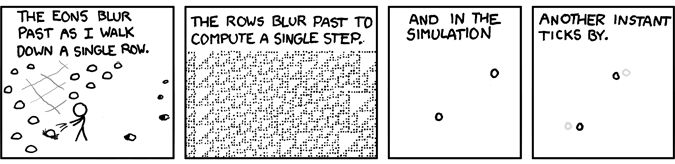
\includegraphics[width=0.75\textwidth]{Images/xkcd/xkcd7.png}
    \caption*{\hspace{\stretch{1}}  Randall Munroe, \emph{A Bunch of Rocks} (part 7 of 9), \texttt{xkcd.com/505/} }
\end{figure}


In free space, two non-interacting and non-identical atoms immersed in a laser field will never be excited simultaneously. This results from a destructive interference phenomenon in the two-photon absorption process of the two atoms in the laser. The two quantum paths underlying the double excitation (one atom excited first, then the second, and vice-versa) interfere destructively precisely when the laser frequency matches the resonance condition for the excitation of the two atoms~\cite{Kim98}. This interference effect can be interestingly annulled if the two atoms are within a distance much smaller than the wavelength of the transition~\cite{Var92, Orr02, Het02}. In this case dipole-dipole interaction comes into play and breaks the destructive character of the interference, resulting in a possible simultaneous excitation of the two atoms.

In Ref.~\cite{Kim98}, the indirect interaction between two atoms placed in a lossless single mode cavity is exploited to obtain a similar cancellation of the destructive interference effect. Here, we wish to extend significantly that initial proposal by considering the huge potentialities offered by circuit-QED systems. Our model is intended to provide realistic experimental predictions by considering dissipation and steady-state regimes using a driving field. A perturbative approach is first proposed to grasp the essentials of the underlying physics in an idealized case.

The organization of the chapter is as follows. In Section~\ref{sec-free}, we introduce the free space case for future comparison with the cavity case and show why simultaneous excitation is not possible in free space. In Sec.~\ref{sec-QEDMod} we give our Hamiltonian for the atoms imbedded in the cavity which includes the modelization of  two internal  states and transitional frequency for each atom, the electromagnetic field mode of the cavity, the coupling between the atoms and the field and finally the driving laser field. We also introduce the master equation which modelizes spontaneous emission or dissipation effects in the atoms as well as the photon loss of the cavity.

In Sec.~\ref{sec-delta}, we introduce a constraint that allows the diagonalization of the undriven Hamiltonian. Thanks to the diagonalization we are able to understand the structure of the dressed states and we can use perturbation theory to predict two-photon transition rates in the system. Then, after discussing some numerical issues, we study one and two-photon spectra as well as the population of the excited atoms in the steady states of the system numerically found with the master equation. We study some effects of the cavity decay rate that could not be including in the perturbation theory analysis.

In Sec.~\ref{sec-phi}, we drop the constraint previously used, which lifts degeneracies, and although we lose the analytical description of the system (except for the particular case of identical atoms) we still use the master equation to calculate  atomic, one and two-photon spectra of the system. We compare the general system with the constrained one and confirm several observations. We also observe a new effect in the system, the cavity induced transparency.

In Sec.~\ref{sec-QEDconcl}, we give a summary of all the theoretical predictions we could make and we discuss the possibility of experimental observation of said predictions.

\section{Atoms in Free Space} \label{sec-free}

Before considering two atoms immersed in a cavity and two-photon processes, we first consider the problem of two atoms in free space excited by a laser and show that in that kind of system, two-photon processes are prohibited.

Let us consider two non-interacting atoms with internal levels $\ket{e_i}$ and $\ket{g_i}$ ($i=1,2$) of transition frequency $\omega_1$ and $\omega_2$ and single atom spontaneous emission rate $2 \gamma_i$. They are excited by a non-resonant laser field of wave vector $\mathbf k_L$, Rabi frequency $2\epsilon$ and driving frequency $\omega$. The Hamiltonian $H_f$  of the system, where $f$ stands for \emph{free}, is
\[ H_f = \sum_{i=1}^2 \left( \hbar (\omega_i-\omega) \sigma^{z}_i +   \hbar \epsilon \left(e^{i \mathbf k_L \cdot \mathbf x_i} \sigma^+_i +e^{-i \mathbf k_L \cdot \mathbf x_i} \sigma^-_i    \right) \right), \]
where $\sigma_i^+ = (\sigma_i^-)^{\dagger}$ is the atom raising operator $\ketbra{e_i}{g_i}$ and $\sigma_i^z$ the atomic inversion operator $(\ketbra{e_i}{e_i}-\ketbra{g_i}{g_i})/2$. We assume that the atoms are placed such that $\mathbf k_L \cdot \mathbf x_1 = \mathbf k_L \cdot \mathbf x_2 = 0$.

When considering dissipation in the Markov and Born approximation, the time evolution of the system is governed by the master equation
\begin{equation}
    \dot\rho = - \frac{i}{\hbar} [H,\rho] -  \sum_{i=1}^2 \gamma_i (\sigma_i^+ \sigma_i^- \rho +\rho \sigma_i^+ \sigma_i^- -2 \sigma_i^- \rho \sigma_i^+), \label{eq-MEFS}
\end{equation}

We now treat the laser as a perturbation by considering a small $\epsilon$.
According to Fermi's Golden Rule of the standard second-order perturbation theory~\cite{Lou00}, the $\ket{gg} \rightarrow \ket{ee}$ transition rate through a strict two-photon process reads
\[ R_{gg \rightarrow ee} = \frac{2 \pi}{\hbar^4}  |W^{(2)}_{(gg,ee)}|^2 \delta(\omega_1+\omega_2 - 2\omega), \]
with
\[ W^{(2)}_{(gg,ee)} = \sum_{j=eg,ge} \frac{ \prodsc{ee}{H}{j}\prodsc{j}{H}{gg} }{\omega_j-\omega}, \]
where here the sum is restricted to the one-excitation $\ket{eg}$ and $\ket{ge}$ states, since they are the only ones to be simultaneously coupled by the perturbation to the $\ket{gg}$ and $\ket{ee}$ states.

Calculating $W^{(2)}_{(gg,ee)}$ is straightforward, we find
\bea
W^{(2)}_{(gg,ee)} &=& \frac{ \prodsc{ee}{H}{eg}\prodsc{eg}{H}{gg} }{\omega_1-\omega}+ \frac{ \prodsc{ee}{H}{ge}\prodsc{ge}{H}{gg} }{\omega_2-\omega}, \\
&=&  \frac{\hbar^2 \epsilon^2}{\omega_1-\omega}+ \frac{\hbar^2 \epsilon^2 }{\omega_2-\omega}, \\
&=& \hbar^2 \epsilon^2  \frac{2 \omega- \omega_1 - \omega_2}{(\omega_1 - \omega)(\omega_2 - \omega)},
\eea
which is equal to zero  when $2 \omega = \omega_1 + \omega_2$. We can see that, due to the destructive interference between the two possible excitation paths $\ket{gg} \rightarrow \ket{eg} \rightarrow  \ket{ee}$ and $\ket{gg} \rightarrow \ket{ge} \rightarrow  \ket{ee}$, the simultaneous excitation of both atoms is prohibited.

The system in its steady state can be can be found posing that the master equation (\ref{eq-MEFS}) is zero. The system can actually be decomposed in two subsystems whose master equation can be solved individually. The steady state solution of two atoms excited in free space is
\[ \rho^S_f = \rho^S_1 \otimes \rho^S_2, \]
with
\[ \rho^S_i = \frac{1}{2\epsilon^2+ \gamma_i^2 + (\omega_i-\omega)^2} \left( \ketbra{\phi_i}{\phi_i} + \epsilon^2 \ketbra{g_i}{g_i}\right), \]
with the unnormalized
\[ \ket{\phi_i} = \epsilon \ket{e_i} - (\omega_i-\omega + i \gamma) \ket{g_i}.\]

The populations of each excited atoms are
\[ P_{e_i} =  \frac{\epsilon^2}{2\epsilon^2+ \gamma_i^2 + (\omega_i-\omega)^2} , \]
and the population in the $\ket{ee}$ state is $P_{ee}= P_{e_1}  P_{e_2}$ since the atoms are independent.

\begin{figure}
    \center
    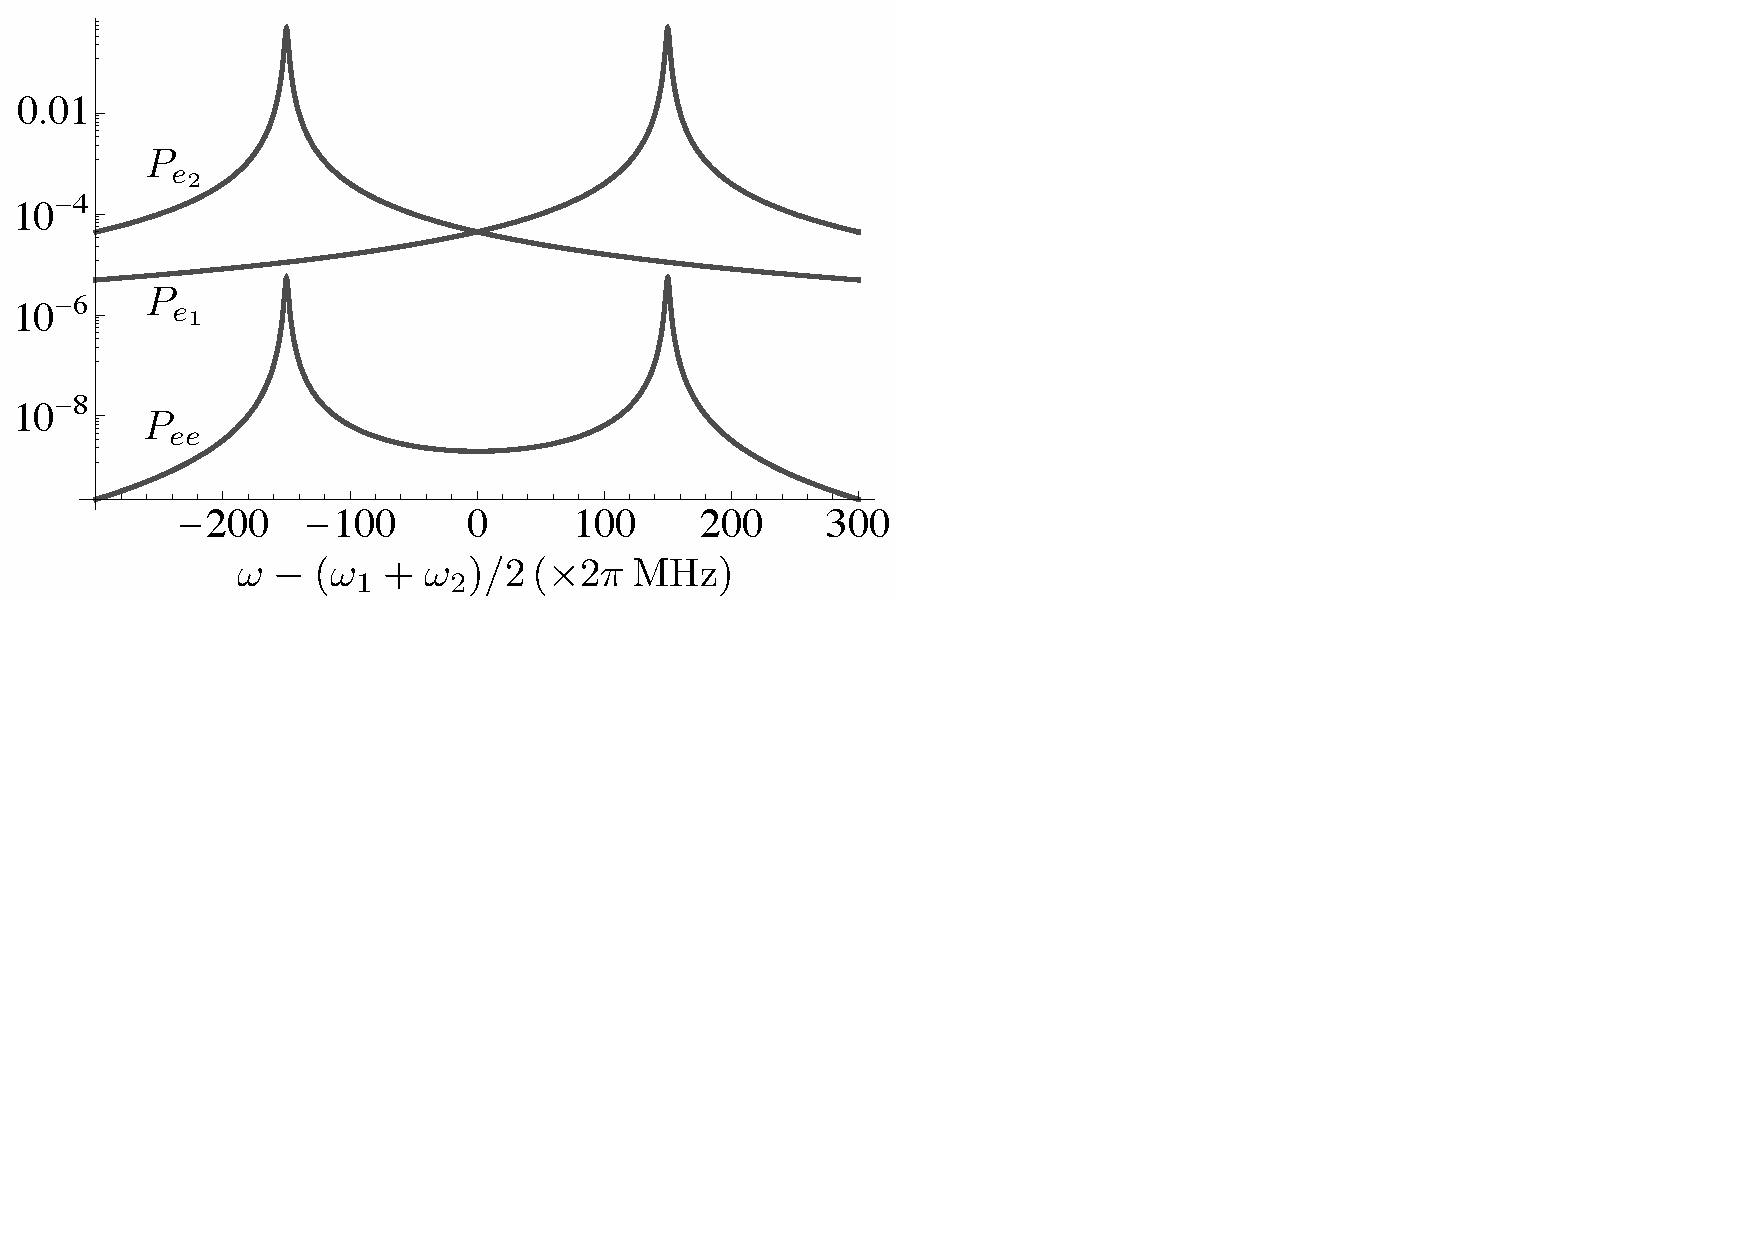
\includegraphics[width=0.65\textwidth]{Images/chap5/free.pdf}
    \caption[Populations in the steady-state]{Populations of $\ket{e_1}, \ket{e_2}$ and $\ket{ee}$ in the steady state with $(\omega_1 - \omega_2)/2 = 150 \times 2\pi\,\mbox{MHz}, \epsilon=2\pi\,\mbox{MHz}, \gamma=0.2  \times 2\pi\,\mbox{MHz}$. There are two peaks located at the frequencies of the individual atoms and none at the frequency $2 \omega = \omega_1 + \omega_2$.}
    \label{fig-free}
\end{figure}

We represented in Fig.~\ref{fig-free} those populations. We see that there is no particular peak at the two-photon transition frequency $2\omega$, which was expected since due to the interference, there can be no two-photon process there. The numerical values and units do not actually apply to real atomic frequencies, but rather to superconducting qubits frequencies existing in circuit QED experiments, as in~\cite{Fin09}. Such qubits are modelized exactly the same way as two-level atoms and are easily manipulated when embedded in a microwave resonator, which is the setup we investigate in the rest of the chapter.

It has been shown that some kind of interaction may counteract the interference and allow two-photon processes to happen\cite{Var92}. In the next sections, we investigate the possibility of allowing two-photon processes by immersing the atoms in a cavity and letting them interact through the cavity coupling.

\section{Atoms Embedded in a Cavity} \label{sec-QEDMod}

We now consider two atoms 1 and 2 with internal levels $\ket {e_i}$ and $\ket{g_i}$ ($i=1,2$) of transition frequency $\omega_i$ and spontaneous emission rate $2\gamma$ (identical for both atoms). The two atoms are embedded in a single mode cavity of resonance frequency $\omega_c$ and decay rate $2\kappa$. The two atoms are supposed to be identically coupled to the cavity with a coupling constant $\alpha$. The cavity is driven by a non-resonant laser field of amplitude $\epsilon$ and driving frequency $\omega$ (see Fig.~\ref{fig-setup}). The two atoms are considered sufficiently far apart so that there is no direct interaction of any kind between them but through the cavity coupling. That situation is encountered in most circuit-QED systems, like, e.g., in the experimental setup reported in Ref.~\cite{Fin09} where the qubits are several hundred micrometers apart.

\begin{figure}
    \center
    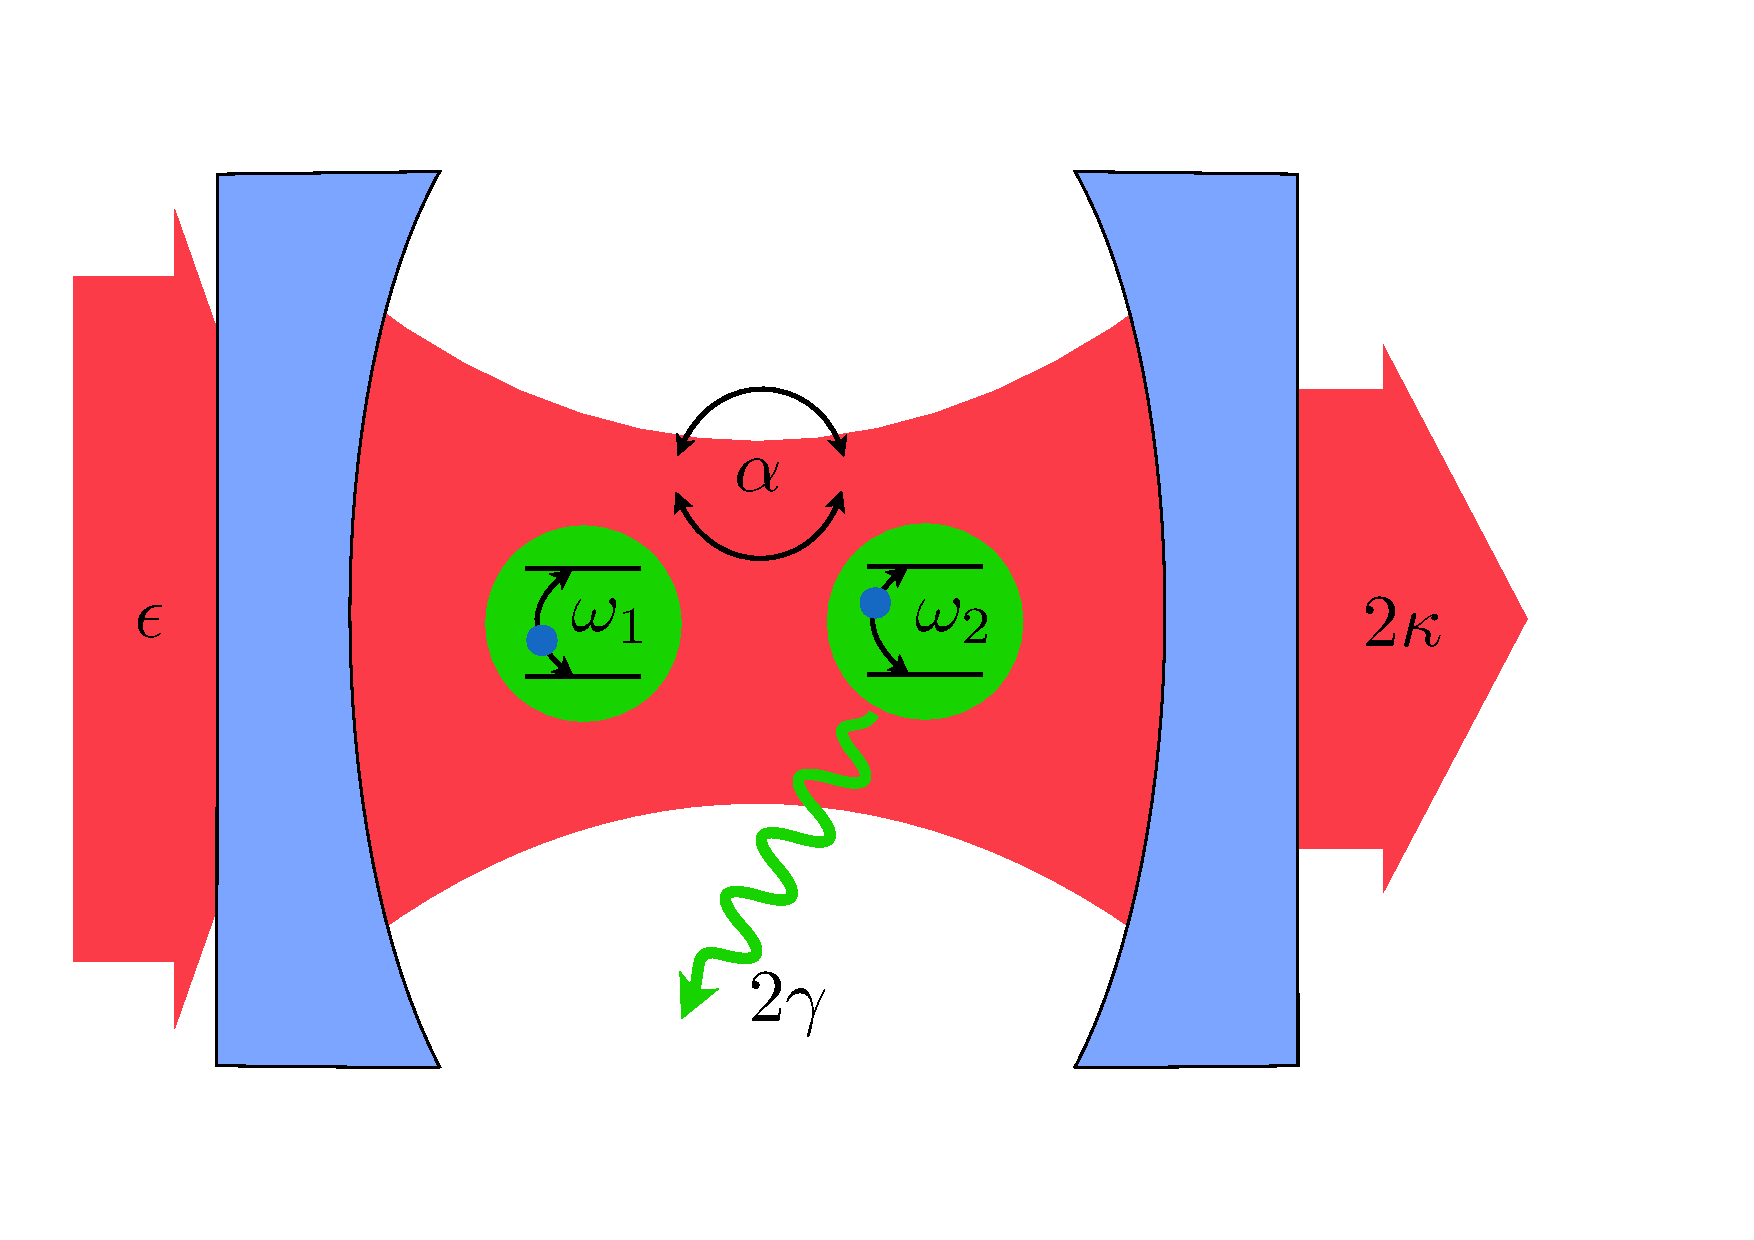
\includegraphics[width=0.5\textwidth]{Images/chap5/setup.pdf}
    \caption[Schematic of the two-atom system]{Schematic of the two-atom system immersed in a single-mode cavity. Two two-level atoms of transition frequencies $\omega_1$ and $\omega_2$ are identically coupled to the cavity mode of frequency $\omega_c$ with a coupling constant $\alpha$. The cavity has a photon decay rate $2\kappa$, while the atoms have a spontaneous emission rate $2\gamma$. The cavity mode is being driven by a laser of strength $\epsilon$ and frequency $\omega$.}
    \label{fig-setup}
\end{figure}

In the rotating-wave approximation, the coherent evolution of the system is described by the interaction Hamiltonian
\[ H = \hbar (\omega_c - \omega) a^\dagger a + \sum_{i=1}^2 \hbar (\omega_i-\omega) \sigma^{z}_i + \sum_{i=1}^2 \hbar \alpha (a \sigma^+_i+a^\dagger \sigma^-_i) + i \hbar \epsilon(a^\dagger - a) , \label{eq-H}\]
where $a$ [$a^\dagger$] is the photon annihilation [creation] operator for the cavity field mode, $\sigma_i^+ = (\sigma_i^-)^{\dagger}$ ($i = 1,2$) is the atom raising operator $\ketbra{e_i}{g_i}$, and $\sigma_i^z$ is the atomic inversion operator $(\ketbra{e_i}{e_i}-\ketbra{g_i}{g_i})/2$.

When considering dissipation in the Markov and Born approximation, the time evolution of the density operator $\rho$ of the system is governed by the master equation~\cite{Aga74}
\[ \dot \rho= \frac{1}{i \hbar} [H,\rho] - \kappa(a^\dagger a  \rho - 2 a\rho a^\dagger +\rho a^\dagger a )  -  \sum_{i=1}^2 \gamma (\sigma_i^+ \sigma_i^-  \rho - 2 \sigma_i^-\rho \sigma_i^+ + \rho \sigma_i^+ \sigma_i^- ).
    \label{eq-MEQED}\]
This time evolution leads invariably to a steady-state $\rho^S$ of the system that is determined by equating the left-hand side term of Eq.~(\ref{eq-MEQED}) to zero. We denote hereafter by $\ket{N,xy} \equiv \ket{N} \otimes \ket{x_1} \otimes \ket{y_2}$ the bare basis elements of the atom-cavity system, with $N$ the photon number and $x,y \in \{e,g\}$.

First, we may want to study the Hamiltonian of the system using a perturbative approach to grasp the essentials of the physics of the system. The driving laser field defines the perturbation and the unperturbed Hamiltonian is given by Eq.~(\ref{eq-H}) with $\epsilon$ and $\omega$ set to 0. Let us show that $H$ commutes with the global excitation number operator $\hat n \equiv a^{\dagger} a + \sum_i \sigma_i^z + 1$, which counts the number of photons in the system plus the number of excited atoms. Obviously, $\hat n$ commutes with the first two terms of the Hamiltonian, we are left with
\bea
[\hat n, H] &=& [a^{\dagger} a + \sum_i \sigma_i^z,  \hbar \alpha \sum_i (a \sigma^+_i+a^\dagger \sigma^-_i)] , \\
&=&  \hbar \alpha \sum_i [a^{\dagger} a,  a \sigma^+_i+a^\dagger \sigma^-_i] + \hbar \alpha \sum_i  [ \sigma_i^z,  a \sigma^+_i+a^\dagger \sigma^-_i],  \\
&=&   \hbar \alpha \sum_i \left(  -a \sigma^+_i+a^\dagger \sigma^-_i \right) + \hbar \alpha \sum_i  \left( a \sigma^+_i- a^\dagger \sigma^-_i \right), \\
&=&0,
\eea
where we used the properties $ [a^{\dagger} a,  a]= [a^{\dagger},  a] a = - a$, $ [a^{\dagger} a,  a^\dagger]= a^\dagger [a,a^{\dagger}]  =  a^\dagger$ and $ [ \sigma_i^z,  \sigma^\pm_j]= \pm \delta_{ij} \sigma^\pm_i$.  It follows that in the $\ket{N,xy}$ bare basis of the atom-cavity system, the unperturbed Hamiltonian has a block-diagonal form, with blocks associated with the global excitation number $n = N + m(x,y)$, where $m(x,y)$ is the number of excited atoms in the $\ket{x,y}$ state ($m = 0$, $1$, or $2$).

For $n=0$, the dimension of the diagonal block is $1 \times 1$, in association with the only bare basis element $\ket{0} \equiv \ket{0,gg}$. For $n=1$, the diagonal block is of $3 \times 3$ dimension with the 3 basis elements $\ket{1,gg}$, $\ket{0,eg}$, and $\ket{0,ge}$. From $n \ge 2$, the diagonal blocks are of $4 \times 4$ dimension in association with the 4 basis elements $\ket{n,gg}$, $\ket{n-1,eg}$, $\ket{n-1,ge}$, and $\ket{n-2,ee}$. The eigenstates and eigenvalues of the unperturbed Hamiltonian yield, respectively, the dressed states of the two-atom-cavity system and their energy. They follow immediately from the block diagonalization.

\section{Even Atomic Frequency Spread}  \label{sec-delta}

The diagonalization of the unperturbed Hamiltonian is possible to realize analytically if we make the assumption that
\[ \omega_1 + \omega_2 = 2 \omega_c, \]
in which case we define the frequency difference $\Delta \equiv (\omega_1-\omega_2)/2$. This means that the frequencies of the atoms are evenly spread around the cavity mode frequency, at the frequencies $\omega_c \pm \Delta$.

\subsection{Eigenstates and Eigenvalues}

Let us now show the results of the block diagonalizations. For $n=0$, $\ket{0}$ is the only eigenstate with an eigenvalue 0. For $n \geq 1$, the eigenvalues read with respect to the ground state energy

\begin{equation}
    \hbar \lambda^{(n,0)} = n \hbar \omega_c, \quad \hbar \lambda^{(n,\pm)} = n \hbar \omega_c \pm \hbar \lambda_n,
\end{equation}
with $\hbar \lambda^{(n,0)}$ twice degenerated for $n \geq 2$ and where
\begin{equation}
    \lambda_n = \sqrt{ 2(2n-1) \alpha^2 + \Delta^2}.
\end{equation}

For $n=1$, the three associated eigenvectors are, respectively,
\begin{align}
    \ket{1,0}   & = \frac{1}{\lambda_1} \left( \Delta \ket{1,gg}  - \sqrt{2} \alpha \ket{\psi^-_1} \right),                                     \\
    \ket{1,\pm} & = \frac{1}{\sqrt{2} \lambda_1} \left(\sqrt 2 \alpha \ket{1,gg} + \Delta \ket{\psi^-_1} \pm \lambda_1 \ket{\psi^+_1} \right) ,
\end{align}
and, for $n \geq 2$, respectively,
\begin{align}
    \ket{n,0_a} & = \sqrt{\frac{n-1}{2n-1}} \ket{n,gg} - \sqrt{\frac{n}{2n-1}} \ket{n-2,ee},                                                              \\
    \ket{n,0_b} & = \frac{1}{\lambda_n} \left( \Delta \ket{\phi_n}  - \sqrt{2(2n-1)} \alpha \ket{\psi^-_n} \right),                                       \\
    \ket{n,\pm} & =  \frac{1}{\sqrt 2 \lambda_n} \left( \sqrt{2(2n-1)} \alpha \ket{\phi_n} +  \Delta \ket{\psi^-_n} \pm \lambda_n \ket{\psi^+_n} \right),
\end{align}
with, for $n \geq 1$,
\begin{equation}
    \ket{\psi^{\pm}_n} = \frac{1}{\sqrt{2}} \left( \ket{n-1,eg} \pm \ket{n-1,ge} \right),
\end{equation}
and, for $n \geq 2$,
\begin{equation}
    \ket{\phi_n} = \sqrt{\frac{n}{2n-1}} \ket{n,gg} +\sqrt{\frac{n-1}{2n-1}} \ket{n-2,ee}. \\
\end{equation}

\begin{figure}
    \center
    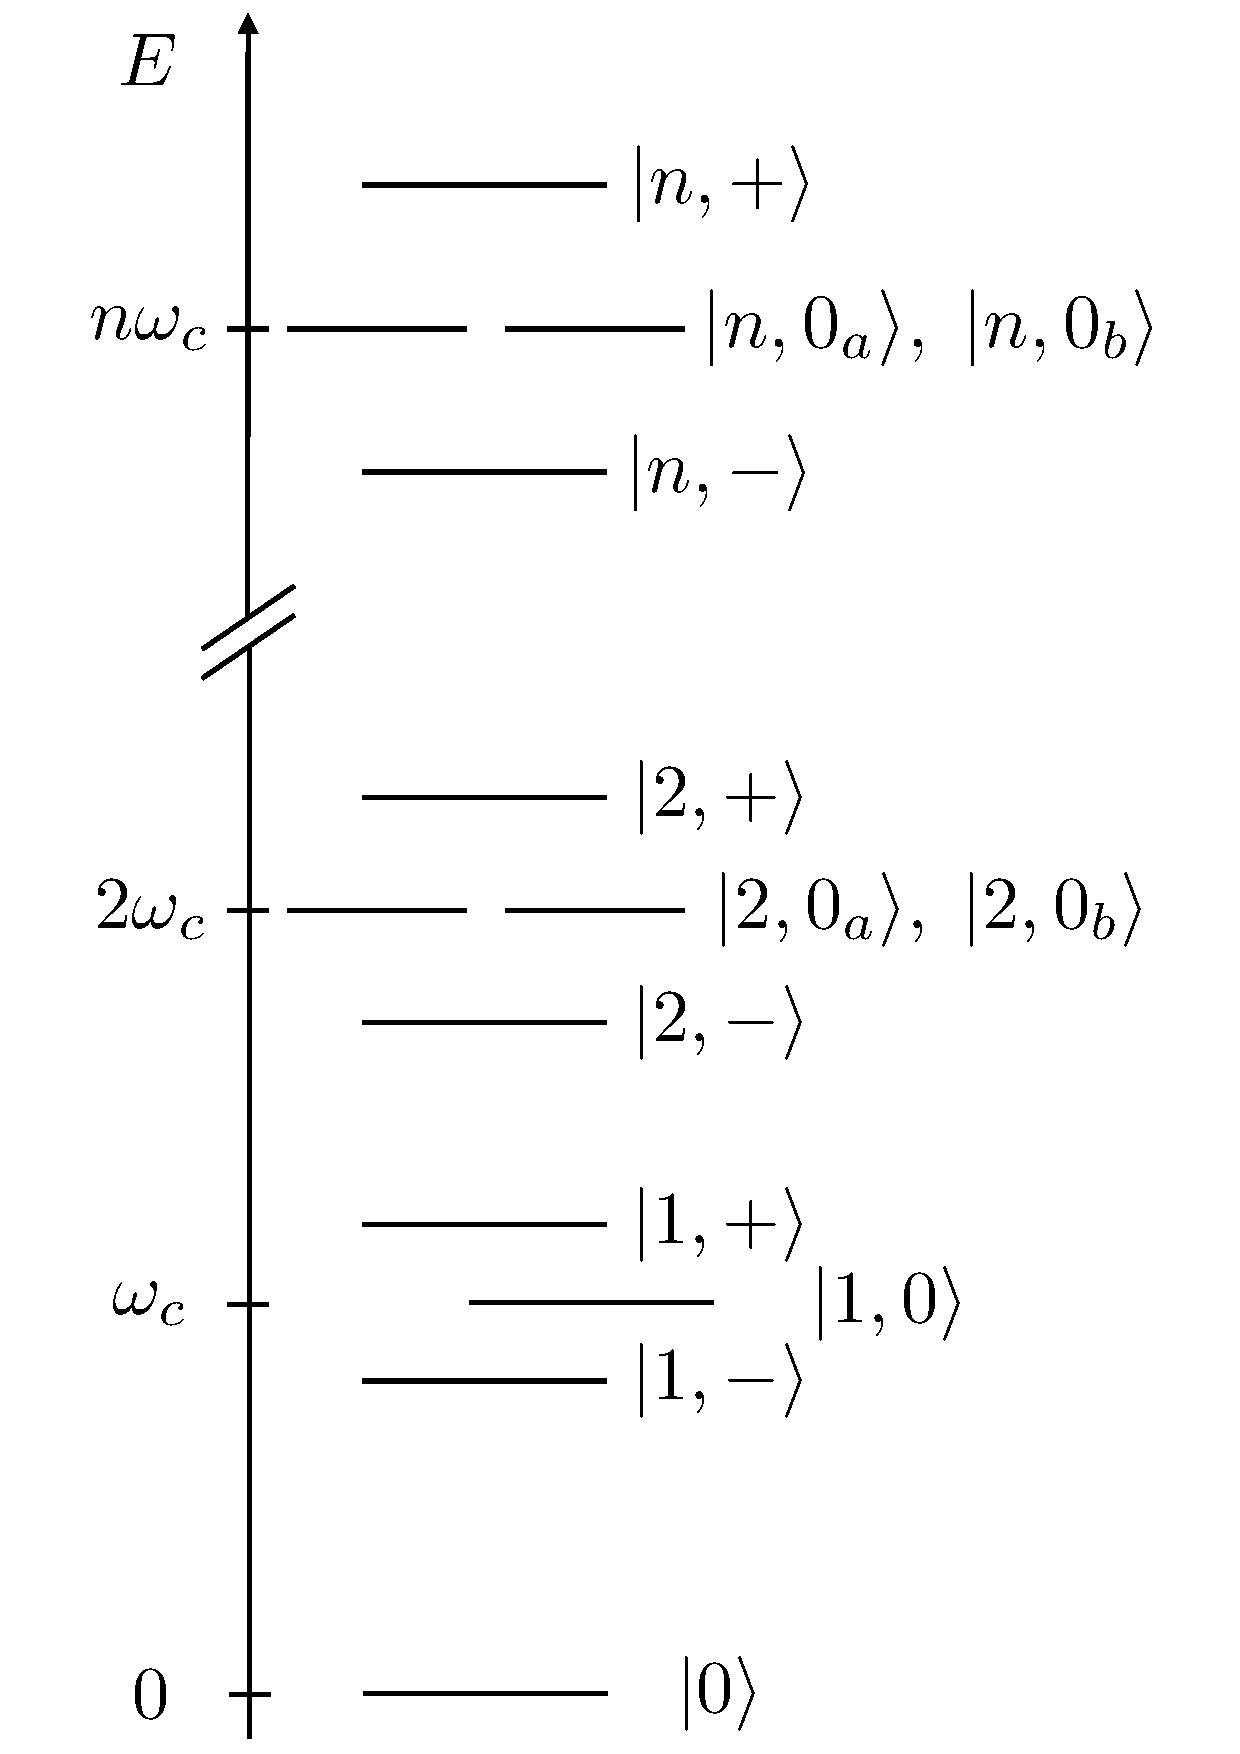
\includegraphics[height=0.4\textheight]{Images/chap5/Energies.pdf}
    \caption[Energy diagram for the dressed states]{Energy diagram for the dressed states of the two-atom-cavity system when $\omega_1+\omega_2 = 2 \omega_c$.}
    \label{fig-eigenvalues}
\end{figure}

The energy structure is shown on Fig.~\ref{fig-eigenvalues}. If we turn on the laser perturbation term $W$ of the Hamiltonian defined as
\[ W = i \hbar \epsilon(a^\dagger - a), \]
the structure of $H$ ceases to be diagonal in the eigenstate basis. The off-diagonal, perturbation terms coming from the laser are expressed, in the unperturbed Hamiltonian eigenstates base, as, for the $n=0 \rightarrow n=1$ transitions
\bea
\prodsc{0}{W}{1,0} &=& -i \,\frac{\Delta}{\lambda_1} \,\epsilon,\\
\prodsc{0}{W}{1,\pm} &=&   -i  \,\frac{\alpha}{\lambda_1}\,\epsilon.
\eea

The $n=1 \rightarrow n=2$ transitions are written
\bea
\prodsc{1,0}{W}{2,0_a} &=& -i\sqrt{\frac{2}{3}}\,\frac{\Delta}{\lambda_1}\,\epsilon ,\\
\prodsc{1,0}{W}{2,0_b} &=& - \frac{2i}{\sqrt 3} \,\frac{3 \alpha^2 + \Delta^2}{\lambda_1 \lambda_2}\,\epsilon ,\\
\prodsc{1,0}{W}{2,\pm} &=& -i \,\frac{\alpha \Delta}{\lambda_1\lambda_2} \,\epsilon,\\
\prodsc{1,\pm}{W}{2,0_a} &=& -i \sqrt{\frac{2}{3}} \,\frac{\alpha}{\lambda_1} \,\epsilon,\\
\prodsc{1,\pm}{W}{2,0_b} &=& \frac{i}{\sqrt 3} \,\frac{\alpha \Delta}{\lambda_1 \lambda_2} \,\epsilon ,\\
\prodsc{1,\pm}{W}{2,\pm} &=& - \frac{i}{4}\,\frac{ (\lambda_1+\lambda_2)^2}{\lambda_1 \lambda_2}\,\epsilon ,\\
\prodsc{1,\pm}{W}{2,\mp} &=&- \frac{i}{4} \,\frac{(\lambda_1-\lambda_2)^2}{\lambda_1 \lambda_2}\,\epsilon.
\eea

Finally, the $n \rightarrow n+1$ transitions with $n\ge 2$ are written
\bea
\prodsc{n,0_a}{W}{n+1,0_a} &=& -2 i  \sqrt{ \frac{n(n^2-1)}{4n^2-1}} \,\epsilon ,\\
\prodsc{n,0_a}{W}{n+1,0_b} &=& -i \sqrt{ \frac{n-1}{4n^2-1}} \,\frac{\Delta}{\lambda_{n+1} } \,\epsilon  ,\\
\prodsc{n,0_a}{W}{n+1,\pm} &=& -i \sqrt{ \frac{n-1}{2n-1}} \,\frac{\alpha}{\lambda_{n+1} }  \,\epsilon,\\
\prodsc{n,0_b}{W}{n+1,0_a} &=&  -i \sqrt{ \frac{n+1}{4n^2-1}} \,\frac{\Delta}{\lambda_{n} } \,\epsilon,\\
\prodsc{n,0_b}{W}{n+1,0_b} &=&  -i \sqrt{ \frac{n}{4n^2-1}} \,\frac{ (n+1)  \lambda_{n}^2 + (n-1)  \lambda_{n+1}^2 }{\lambda_n \lambda_{n+1} } \,\epsilon,\\
\prodsc{n,0_b}{W}{n+1,\pm} &=&  -i \,\frac{\alpha \Delta }{\lambda_n \lambda_{n+1} } \,\epsilon,\\
\prodsc{n,\pm}{W}{n+1,0_a} &=& -i  \sqrt{ \frac{n+1}{2n+1}} \,\frac{\alpha}{\lambda_n } \,\epsilon,\\
\prodsc{n,\pm}{W}{n+1,0_b} &=& i  \sqrt{ \frac{n}{2n+1}} \,\frac{\alpha \Delta }{\lambda_n \lambda_{n+1} } \,\epsilon,\\
\prodsc{n,\pm}{W}{n+1,\pm} &=&  -i \frac{\sqrt{n}}4 \,\frac{(\lambda_n+\lambda_{n+1})^2}{\lambda_n \lambda_{n+1}} \,\epsilon,\\
\prodsc{n,\pm}{W}{n+1,\mp} &=&  -i \frac{\sqrt{n}}4 \,\frac{ (\lambda_n-\lambda_{n+1})^2}{\lambda_n \lambda_{n+1}}  \,\epsilon.\\
\eea


From the matrix elements, we identify three one-photon transitions from the ground state at frequencies $\omega_c$ and $\omega_c \pm \lambda_1$ and two two-photon transitions $|0\rangle \rightarrow |2,\pm\rangle$ at frequencies $\omega_c \pm \lambda_2/2$.  Unlike the free space case, the transition at $2\omega=\omega_1+\omega_2=2\omega_c$ which corresponds to $\ket 0 \rightarrow \ket{2,0_{a,b}}$ does not identify as two-photon processes but rather to stepwise one-photon transitions through the intermediate state $\ket{1,0}$ with photons at frequency $\omega_c$.

In general, $n$-photon transitions to the states $\ket{n,\pm}$ at the frequencies $\omega_c \pm \lambda_n/n$ are conceivable, although the transition rates are proportional to $\epsilon^{2n}$ in the perturbation regime.

\subsection{Perturbative Approach}

We now consider the action of the driving field at frequency $\omega$ and investigate the possibility of getting both atoms excited through strict two-photon processes, a result that is not achievable when the two atoms are solely in free space. Here, the two-photon transitions $|0\rangle \rightarrow |2,\pm\rangle$ make this possible because of the $\ket{0,ee}$ component of the upper states $|2,\pm\rangle$.

According to Fermi's Golden Rule of the standard second-order perturbation theory~\cite{Lou00}, the $|0\rangle \rightarrow |0,ee\rangle$ transition rate through a strict two-photon process reads
\[ R_{gg \rightarrow ee} = \frac{2 \pi}{\hbar^4} |\langle 0,ee | 2,\pm \rangle|^2 |W^{(2)}_{0,(2,\pm)}|^2 \delta(\lambda^{(2,\pm)} - 2\omega), \label{eq-Ree}\]
with
\[  W^{(2)}_{0,(2,\pm)} = \sum_{j=0,\pm} \frac{\langle 2,\pm | W |1, j\rangle \langle 1,j | W |0\rangle}{\lambda^{(1,j)}-\omega},\]
where here the sum is only restricted to the one-excitation $\ket{1,j}$ states, since they are the only ones to be simultaneously coupled by the perturbation $W$  to the $|0\rangle$ and $|2,\pm\rangle$ states.

In Eq.~(\ref{eq-Ree}), the $\delta$-function yields the two-photon resonance condition $\omega = \omega_c \pm \lambda_2/2$ that must be fulfilled to get the sought double-excitation process.  Let us first calculate
\bea
\prodsc{2,\pm}{W}{1,0}\prodsc{1,0}{W}{0} &=&  -\frac{\alpha \Delta^2}{\lambda_1^2\lambda_2}  \,\epsilon^2, \\
\prodsc{2,\pm}{W}{1,\pm}\prodsc{1,\pm}{W}{0} &=&- \frac{1}{4}\,\frac{\alpha (\lambda_1+\lambda_2)^2}{\lambda_1^2 \lambda_2} \,\epsilon^2,\\
\prodsc{2,\pm}{W}{1,\mp}\prodsc{1,\mp}{W}{0} &=& - \frac{1}{4}\,\frac{\alpha (\lambda_1-\lambda_2)^2}{\lambda_1^2 \lambda_2} \,\epsilon^2.
\eea

We then have
\bea
W^{(2)}_{0,(2,\pm)}&=& - \frac{\alpha \epsilon^2 }{\lambda_1^2 \lambda_2}\left( \frac{ \Delta^2 }{\omega_c - \omega}+  \frac{(\lambda_1 \pm \lambda_2)^2}{4(\omega_c - \omega +\lambda_1)}+ \frac{(\lambda_1 \mp \lambda_2)^2 }{4(\omega_c - \omega-\lambda_1)} \right), \\
&=& - \frac{\alpha \epsilon^2 }{\lambda_2}\, \frac{ \Delta^2 + (\omega_c - \omega) \left(  \lambda_2 \mp 2 (\omega_c - \omega)\right) }{(\omega_c - \omega)(\omega_c - \omega +\lambda_1)(\omega_c - \omega -\lambda_1)},
\eea
which gives, at the resonance condition $\omega = \omega_c \pm \lambda_2/2$ and after a few simplifications
\begin{equation}
    \label{Pggee2}
    R_{gg \rightarrow ee} = 2 \pi f(r) \frac{\epsilon^4}{\Delta^2} \delta(\lambda^{(2,\pm)} - 2\omega),
\end{equation}
where $r = \alpha/\Delta$ and
\begin{equation}
    f(r) = \frac{2304 r^8}{(1 + 6 r^2)^3 (3 + 2 r^2)^2}.
\end{equation}

As expected, this rate is strongly dependent on the coupling constant $\alpha$ and on the spread $2 \Delta$ in atomic frequencies, but there will be two-photon transitions as long as the atoms are coupled with the cavity. For $r \ll 1$, the rate behaves as $r^8$, while it behaves as $r^{-2}$ for $r \gg 1$. The optimal rate is obtained for $r \sim 1.51$ that yields $2 \pi f(r) \sim 2.16$.

When the atoms are identical, i.~e.~when $\Delta=0$, the $\ket 0 \rightarrow \ket{2,\pm}$ transitions still take place, at the transition rate
\[R_{gg \rightarrow ee} (\Delta=0)= 2 \pi \frac{8 \epsilon^4}{3 \alpha^2} \delta(\lambda^{(2,\pm)} - 2\omega). \]

Let us examine the possible transitions at $\omega=\omega_c$ when the atoms are identical. We note that when this is the case, the system becomes symmetric with the exchange of the two atoms. It is easy to see that the states $\ket{1,0}$ and $\ket{n,0_b}$ are now antisymmetric with the exchange of the atoms while the other states are symmetric. It is apparent from the perturbation terms in the Hamiltonian that the antisymmetric states only couple to each other and are completely decoupled from the symmetric states, including the ground state, and should therefore never be populated. In other words, since $\prodsc{0}{W}{1,0}=0$, the only one-photon transition from the ground state at $\omega=\omega_c$ is impossible. The two-photon process $\ket 0 \rightarrow \ket{2,0_b}$ is also impossible since $W^{(2)}_{0,(2,0_{b})}$ is always zero, as we have $\prodsc{2,0_b}{W}{1,\pm}=0$.

There might still remain the possibility of a transition at $\omega=\omega_c$ if the $\ket{2,0_a}$ state is populated from the ground state by a two-photon process. The rate of this process is proportional to $|W^{(2)}_{0,(2,0_{a})}|^2$, with
\bea
W^{(2)}_{0,(2,0_{b})} &=&  \sum_{j=\pm} \frac{\langle 2,0_b | W |1, j\rangle \langle 1,j | W |0\rangle}{\lambda^{(1,j)}-\omega}, \\
&=&  \frac{ \prodsc{2,0_a}{W}{1,+}\prodsc{1,+}{W}{0} }{\omega_c-\omega + \lambda_1}+  \frac{ \prodsc{2,0_a}{W}{1,-}\prodsc{1,-}{W}{0} }{\omega_c-\omega + \lambda_1}, \\
&=& -\sqrt{\frac{2}{3}} \frac{\alpha^2\epsilon^2}{\lambda_1^2 \lambda_2} \left( \frac{ 1}{\omega_c-\omega + \lambda_1}+  \frac{ 1}{\omega_c-\omega + \lambda_1} \right), \\
&=& -\sqrt{\frac{2}{3}} \frac{\alpha^2\epsilon^2}{\lambda_1^2 \lambda_2} \frac{2( \omega_c-\omega)}{(\omega_c-\omega + \lambda_1)(\omega_c-\omega - \lambda_1)}, \\
\eea
which is always zero on the resonance condition $\omega=\omega_c$. Therefore no transition takes place at the atomic frequencies when they are identical.

Here, we investigated the transition rates for both atoms to simultaneously go from their ground state to their excited state. We may also be interested in the possibility of the number of photons in the cavity going from $N=0$ to $N=2$ instantly. The golden rule (\ref{eq-Ree}) may be modified to calculate such a two-photon process. Since the ground state is the same for atoms or photons, one just needs to replace the $|\langle 0,ee | 2,\pm \rangle|^2$ term which calculates the proportion of $\ket{ee}$ state in $\ket{2,\pm}$ by $\prodsc{2,\pm}{(a^\dagger)^2 a^2}{2,\pm}$ which calculates the number of pairs of photons in $\ket{2,\pm}$. The $W^{(2)}_{0,(2,\pm)}$ needs no modification, therefore all qualitative result on $\ket{gg}\rightarrow \ket{ee}$ also applies to the  photon sates $\ket{N=0}\rightarrow \ket{N=2}$.

\subsection{Master Equation Approach} \label{sec-QEDdiss}

In this section, we refine our analysis by using a more general, although numerical, method to investigate the behavior of the system. A master equation approach is used, into which dissipations such as atomic spontaneous emission and cavity loss are considered. We numerically solve the master equation for the steady state of the system and measure different observables. The results obtained will be interpreted in light of the perturbative approach of the previous section and we will show that two-photon processes are indeed allowed in the present system.

\subsubsection{Numerical Considerations}

Here, we discuss the numerical methods used to calculate the following results. In order to obtain results as realistic as possible, we chose to give to our parameters values close to what has been used in recent circuit QED experiments, as in~\cite{Fin09}. The typical values we used are listed in Tab.~\ref{tab-values}, unless stated otherwise.

\begin{table} \begin{center}
        \caption{Numerical values of the model. }
        \begin{tabular}{c|c}
            Parameter    & Value ($\times 2 \pi$~MHz) \\ \hline \hline
            $\Delta$     & 0, 150                     \\
            ${\alpha}$   & 85                         \\
            ${\epsilon}$ & 6                          \\
            ${\kappa}$   & 6.8                        \\
            ${\gamma}$   & 0.2
        \end{tabular}
        \label{tab-values}
        \caption*{Numerical values used in the numerical processes, unless stated otherwise. }
    \end{center}\end{table}


\begin{table} \begin{center}
        \caption{Other numerical values of the model. }
        \begin{tabular}{c|c}
            Parameter    & Value ($\times 2 \pi$~MHz) \\ \hline \hline
            $\Delta$     & 0, 150                     \\
            ${\alpha}$   & 85                         \\
            ${\epsilon}$ & 6                          \\
            ${\kappa}$   & 6.8                        \\
            ${\gamma}$   & 0.2
        \end{tabular}
        \label{tab-values2}
        \caption*{Numerical values used in the numerical processes, unless stated otherwise. Totally different from the previous table}
    \end{center}\end{table}

Our goal in this chapter is to highlight the two-photon processes, which are proportional to $\epsilon^4$, compared to the one-photon processes, proportional to $\epsilon^2$ in the perturbation regime. With that in mind, it makes sense to choose a high laser power in order to increase the visibility of the two-photon transitions. However, as the strength of the laser probing the system is increased, more and more excitation modes are being populated and for numerical purposes we cannot use an infinite vector basis for the photon number $\ket{N}$. Therefore, we need to make approximations in order to solve the master equation by cutting off the excitation number to a maximum $n_{\mbox{max}}$. Unfortunately, with a truncated basis for high laser power the populations come numerically to a saturation and harmonization of all the different populations in the density matrix. We need a way to evaluate this effect in order to chose a laser power as high as possible which still minimizes numerical errors.

It would possible to estimate the saturation effect in the numerical process by comparing the number of photons calculated for  an empty cavity to the number it should really have, which can be calculated analytically for an infinite basis. Indeed, the master equation relating to  an empty cavity is written
\[\dot \rho= \frac{1}{i \hbar} [H_0,\rho] - \kappa(a^\dagger a  \rho - 2 a\rho a^\dagger +\rho a^\dagger a ), \label{eq-H0}\]
with the excited empty cavity Hamiltonian
\[H_0 =  \hbar (\omega_c - \omega) a^\dagger a + i \hbar \epsilon(a^\dagger - a).  \]

The time variation of any operator $A$ is calculated using Eq.~(\ref{eq-H0}) as
\bea
\frac{d}{dt} \mean{A} &=& \tr{A \dot \rho} , \\
&=&-i(\omega_c - \omega) \tr{ A a^\dagger a \rho -A \rho a^\dagger a} + \epsilon \tr{A a^\dagger \rho-A \rho a^\dagger -A a \rho+ A \rho a} \nonumber \\
&& \  - \kappa \tr{Aa^\dagger a  \rho} + 2 \kappa \tr{A a \rho a^\dagger} -\kappa \tr{A \rho a^\dagger a }, \\
&=&-i(\omega_c - \omega) \mean{[A, a^\dagger a]} + \epsilon \left( \mean{[A, a^\dagger]} - \mean{[A, a]} \right) \nonumber \\
&& \ - \kappa \left( \mean{Aa^\dagger a  - 2 a^\dagger A a + a^\dagger a A }\right), \label{eq-dAdt}
\eea
where we used the invariance of the trace under cyclic permutations of the operators it act on. If we want to calculate the time variation of the mean number of photons, we have $A=a^\dagger a$ and we calculate
\begin{align}
     & [A, a^\dagger a]=0, \;\; [A, a^\dagger ] = a^\dagger [a, a^\dagger ]  = a^\dagger, \;\; [A, a]= -[a, a^\dagger ] a  = a,                              \\
     & Aa^\dagger a  - 2 a^\dagger A a + a^\dagger a A= 2(a^\dagger a a^\dagger a - a^\dagger a^\dagger a a) = 2 a^\dagger [a, a^\dagger] a= 2 a^\dagger a ,
\end{align}
where we used the commutation relation $ [a, a^\dagger ] = 1$. We finally find
\[ \frac{d}{dt} \mean{a^\dagger a} = \epsilon( \mean{a^\dagger}+ \mean{a})  - 2 \kappa \mean{a^\dagger a}.\]

Let us also calculate the time variation of the annihilation operator $A=a$. We have
\begin{align}
     & [A, a^\dagger a]= [a, a^\dagger ] a = -a  , \;\; [A, a^\dagger ] = 1, \;\; [A, a]= 0,                     \\
     & Aa^\dagger a  - 2 a^\dagger A a + a^\dagger a A= a a^\dagger a - a^\dagger a a =  a [a, a^\dagger ] = a ,
\end{align}
and we find
\[ \frac{d}{dt} \mean{a} =  -i(\omega_c - \omega) \mean{a} +\epsilon - \kappa \mean{a}, \]
and $\frac{d}{dt} \mean{a^\dagger}$ is the complex conjugate of $\frac{d}{dt} \mean{a}$.  At the system equilibrium, the time variations are null and as we solve the system we find for the steady state
\[\mean{a^\dagger a} = \frac{\epsilon^2}{\kappa^2 + (\omega_c-\omega)^2}.  \label{eq-QEDempty}\]

Now we can compare the value we numerically obtain from the steady state using a truncated basis to (\ref{eq-QEDempty}) to get an idea of the saturation effect. In this work, we always consider excitation numbers going up to $n_{\mbox{max}}=5$. When the cavity is empty and on resonance, which is obtained by setting $\alpha=0$ and $\omega_c = \omega$, we find, using the parameter values shown in Table~\ref{tab-values}, a difference with Eq.~(\ref{eq-QEDempty}) of $\sim 0.5\%$. We did not use a higher power laser, to prevent going beyond that margin of error.

\subsubsection{One and two-photon Spectroscopy}

The transmission $T$ of an optical cavity of decay rate $\kappa$ is the quantity of photons that filter out of one of the mirrors of the cavity and is given by $T=\kappa \langle a^\dagger a \rangle$. The second order transmission $T^{(2)}$  consider the events involving more than one photon detected at the same time by a photodetector and is given by $T^{(2)}=\kappa^2 \langle (a^\dagger)^2 a^2 \rangle$. In the following section, we study the values of the populations $\langle a^\dagger a \rangle$ and $\langle (a^\dagger)^2 a^2 \rangle$ inside the cavity for the steady state $\rho^S$ in function of the laser frequency $\omega_c$, the transmissions being directly proportional.

\begin{figure}
    \center
    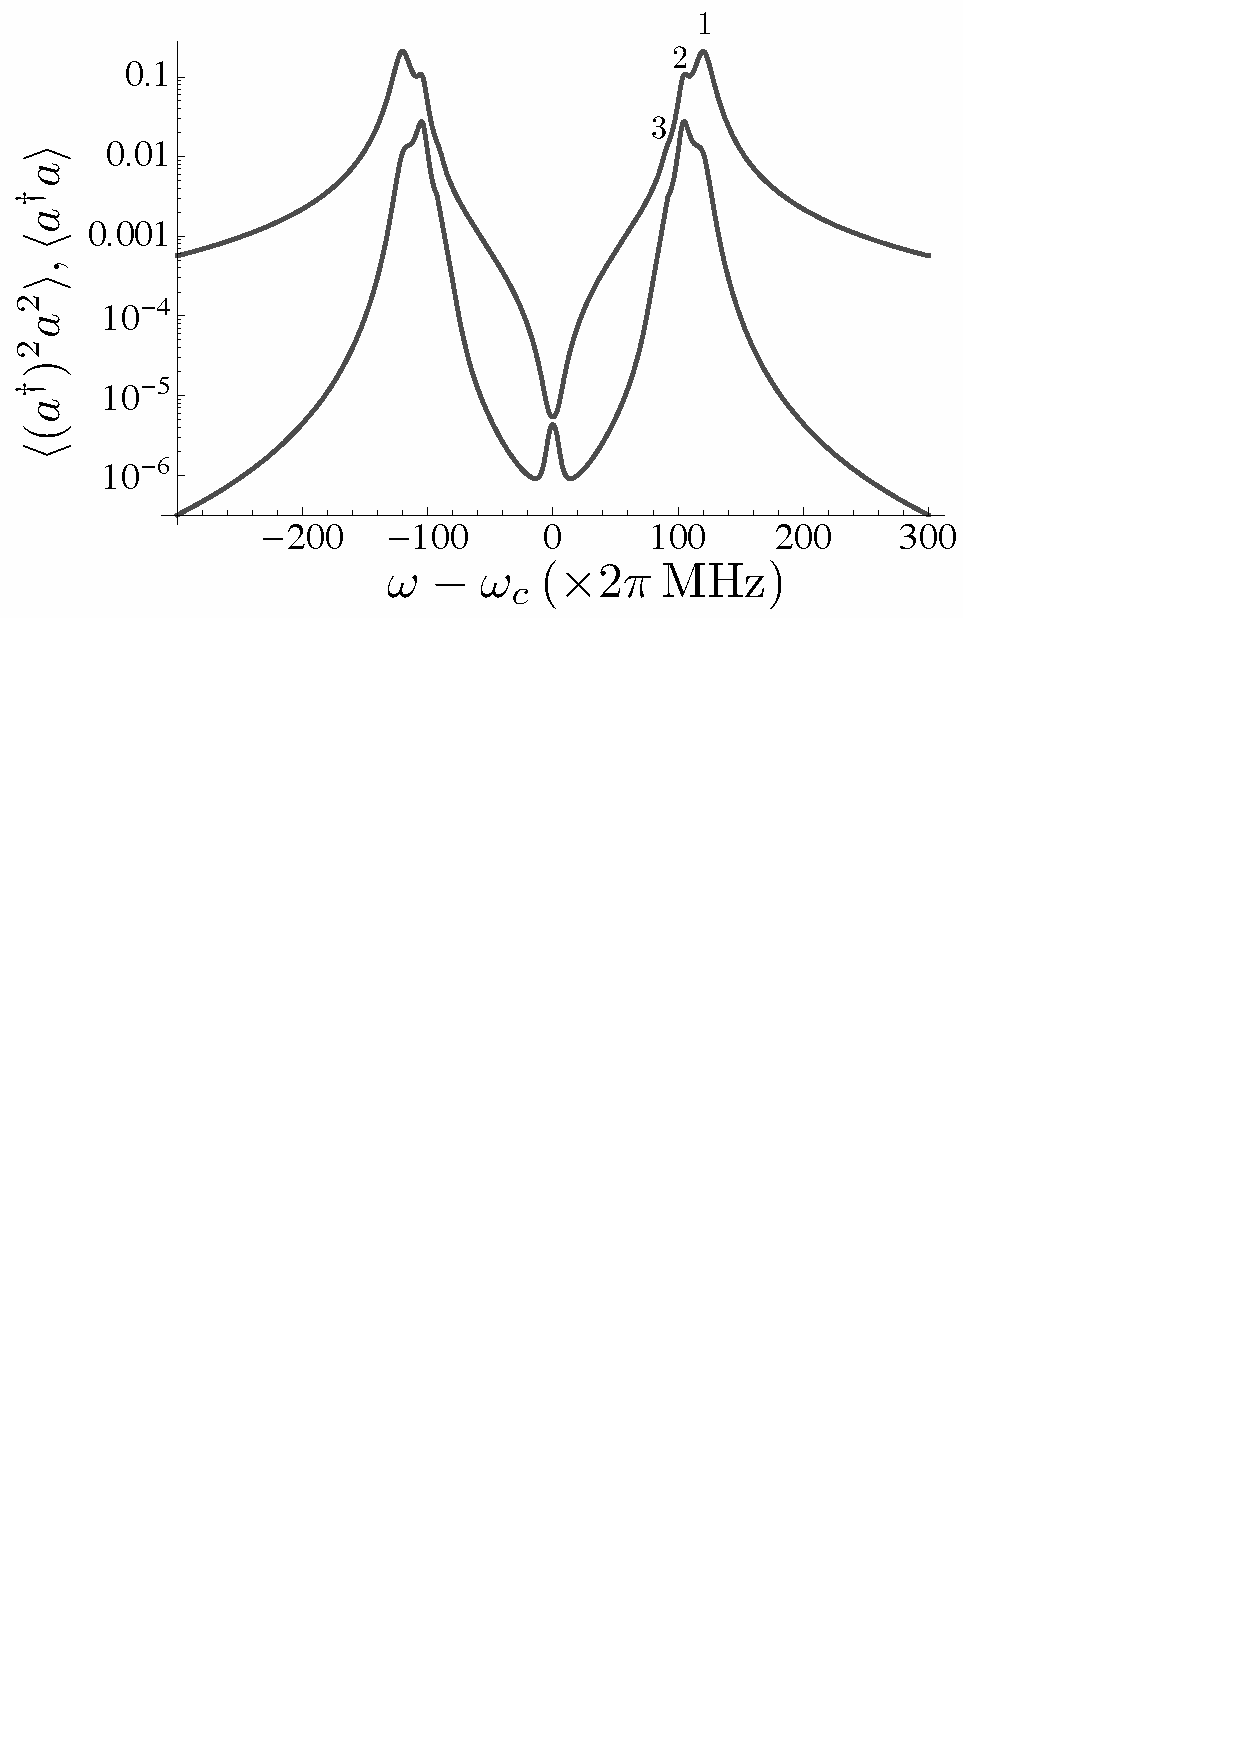
\includegraphics[width=0.75 \textwidth]{Images/chap5/spectrum0.pdf}
    \caption[$\langle a^\dagger a \rangle$ and $\langle (a^\dagger)^2 a^2 \rangle$  in function of  $\omega-\omega_c$]{Spectra of $\langle a^\dagger a \rangle$ (top) and $\langle (a^\dagger)^2 a^2 \rangle$ (bottom) in function of  $\omega-\omega_c$ for the values in Tab.~\ref{tab-values} and $\Delta=0$. Note the absence of peak at $\omega=\omega_c$. The other peaks are numbered as the order of the $n$-photon transition $\ket 0 \rightarrow \ket{n,+}$ at $\omega-\omega_c=\lambda_n/n$: one-photon, two-photon and an embryo of the three-photon transition can be made out. The symmetrical peaks on the left side correspond to the $n$-photon transition $\ket 0 \rightarrow \ket{n,-}$.}
    \label{fig-spec0}
\end{figure}

First we study the resonant case. When the atoms have the same internal frequency than the cavity, i.~e.~when $\Delta=0$, we found that the state $\ket{1,0}$ does not get populated, since $\prodsc{1,0}{W}{0,gg}$ vanishes and neither do the states $\ket{2,0_{a,b}}$. Hence, we should not expect to see a one photon transition peak at the frequency $\omega=\omega_c$. We plotted the photon spectrum in Fig.~\ref{fig-spec0}, and we see that, indeed, on the top curve the photon population at $\omega=\omega_c$ is highly inhibited, the main peaks of the spectrum are those due to the $\ket{n,\pm}$ transitions, for $n=1, 2$ and slightly $n=3$.

We see the peaks due to the one-photon processes $\ket 0 \rightarrow \ket{1,\pm}$ in the $\mean{(a^\dagger)^2 a^2}$ spectrum, but the laser power is strong enough for the amplitude of the two-photon $\ket 0 \rightarrow \ket{2,\pm}$ transition peak to dominate it and to bring a non-negligible contribution in the spectrum of $\mean{a^\dagger a}$.  That dominance grows as the laser power increases, since the $n$ photons transitions rates scale as $\sim \epsilon^{2n}$. We note a small peak at $\omega=\omega_c$ for $\mean{(a^\dagger)^2 a^2}$. That peak might be explained by higher order transitions ($n\ge3$) which are not inhibited, but also not strong enough to show on $\mean{a^\dagger a}$.
%This peak is explained by the fact that the dissipation effects do not follow the symmetry of the Hamiltonian and therefore tend to populate the antisymmetric state $\ket{1,0}$. Once this state is populated, even weakly, the transition $\ket{0,1} \rightarrow \ket{2,0_b}$ happens and populates the twice excited state. However this effect is quite small and does not appear on the spectrum of $\mean{a^\dagger a}$. 

\begin{figure}
    \center
    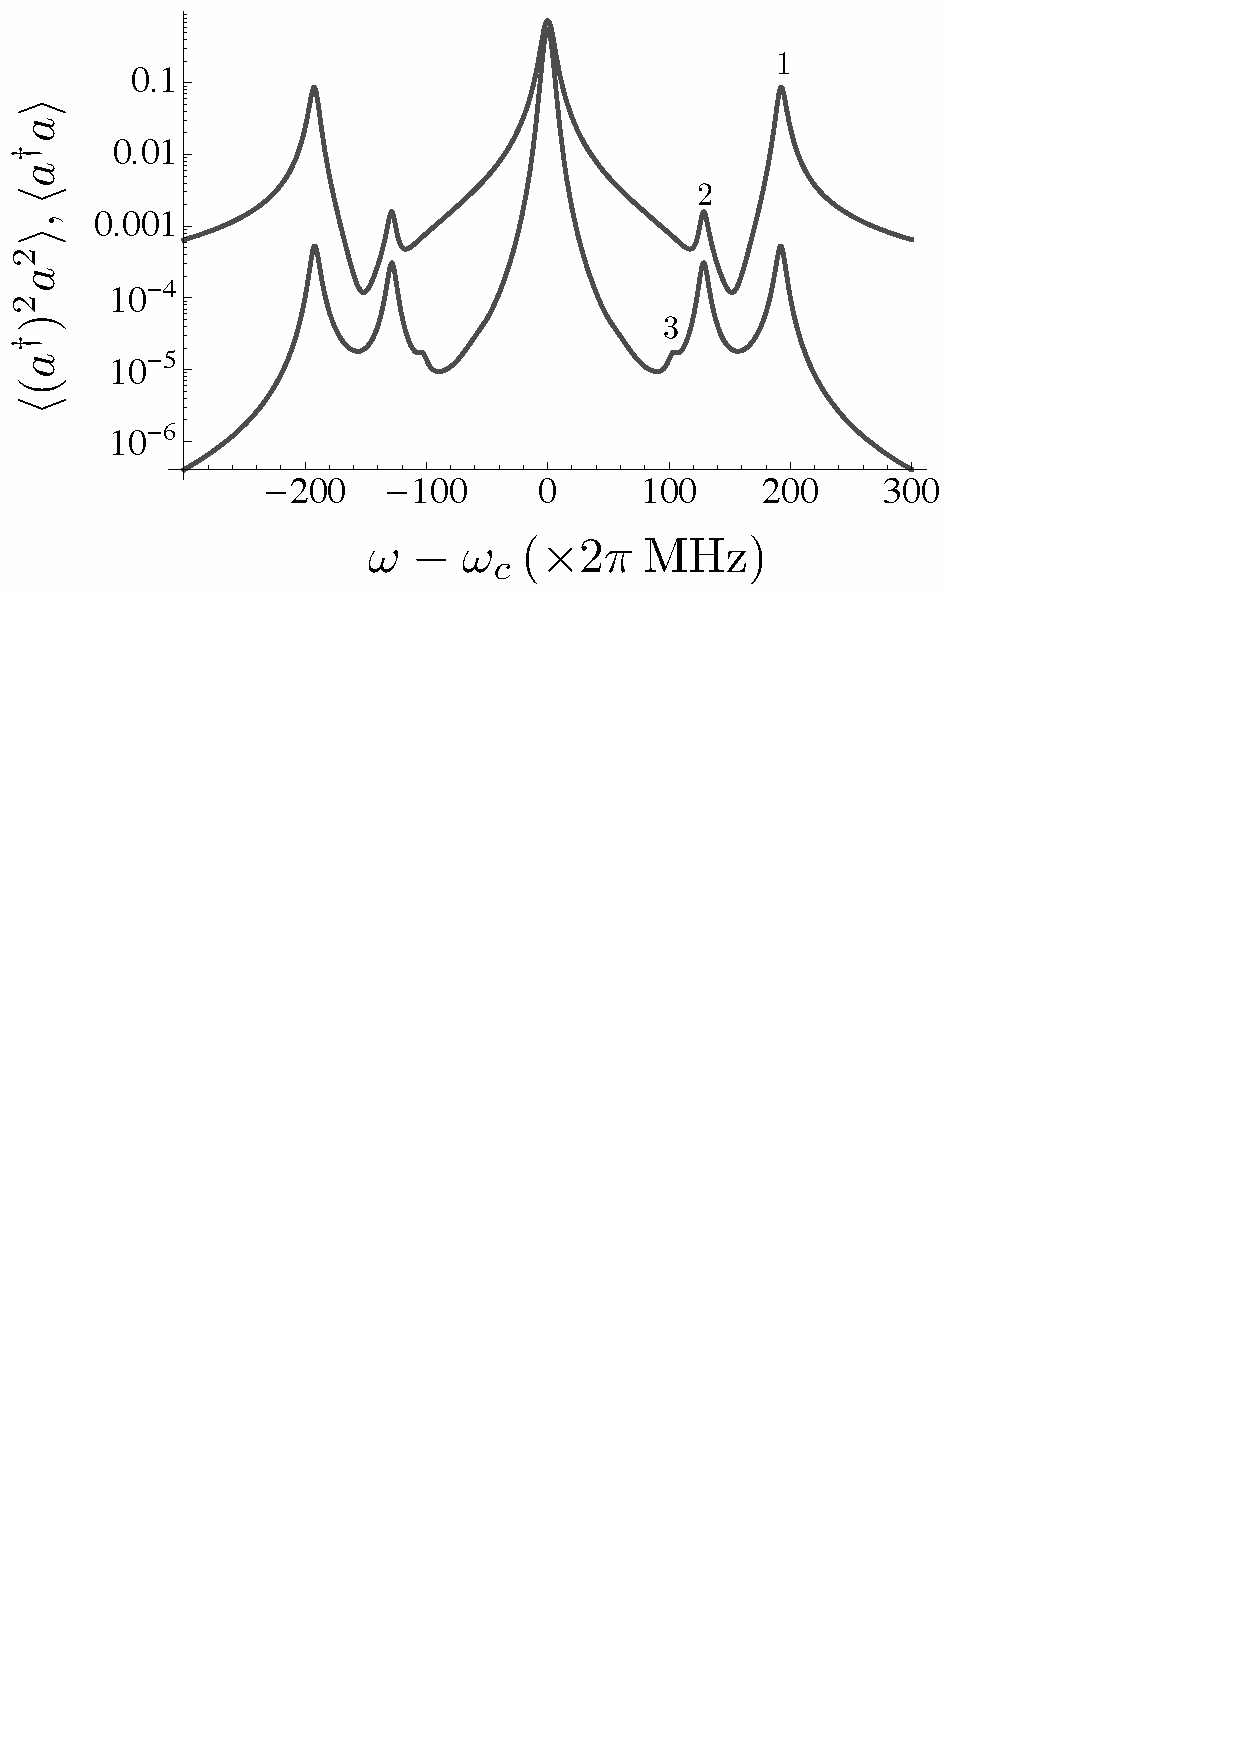
\includegraphics[width=0.75 \textwidth]{Images/chap5/spectrum150.pdf}
    \caption[$\langle a^\dagger a \rangle$ and $\langle (a^\dagger)^2 a^2 \rangle$]{Spectra of $\langle a^\dagger a \rangle$ (top) and $\langle (a^\dagger)^2 a^2 \rangle$ (bottom) in function of  $\omega-\omega_c$ for the values in Tab.~\ref{tab-values} and $\Delta=150 \times 2\pi\,\mbox{MHz}$. The transition at $\omega=\omega_c$ is not inhibited anymore, on the contrary it yields the most important peak. The other peaks are numbered as the order of the $n$-photon transition $\ket 0 \rightarrow \ket{n,+}$ at $\omega-\omega_c=\lambda_n/n$: one-photon, two-photon and three-photon (not visible on the $\mean{a^\dagger a}$ spectrum). The symmetrical peaks on the left side correspond to the $n$-photon transitions $\ket 0 \rightarrow \ket{n,-}$.}
    \label{fig-spec150}
\end{figure}

Then we study the non-resonant case by setting $\Delta=150 \times 2\pi\,\mbox{MHz}$ in Fig.~\ref{fig-spec150}. In that situation, the matrix element $\prodsc{1,0}{W}{0}$ is no longer zero and the transitions at $\omega=\omega_c$ are allowed again, hence the observed peak at the cavity resonance frequency which largely dominates the other transition peaks. The transition at $\omega=\omega_c$ is the condition for the consecutive one-photon transitions $\ket 0 \rightarrow \ket{1,0}\rightarrow \cdots \rightarrow \ket{n,0_{a,b}}$, which is why the peak is also very important on $\mean{(a^\dagger)^2 a^2}$, unlike the peak corresponding to the $\ket 0 \rightarrow \ket{1,\pm}$, which does not correspond to a two-photon process and is henceforth comparatively much weaker on the $\mean{(a^\dagger)^2 a^2}$ spectrum. Once again,  we note that in the two-photon spectrum the two-photon transmission to $\ket{2,\pm}$ is of the same order of magnitude than the transmission to $\ket{1,\pm}$, due to the strength of the laser power. Also, we note the emergence of two new peaks, only visible on $\mean{(a^\dagger)^2 a^2}$, which are due to three-photon transitions.

%\begin{figure}
%\center
%\includegraphics[width=0.75 \textwidth]{Images/chap5/g2.pdf}
%\caption{Spectra of $g^{(2)}(0)$  in function of $\omega-\omega_c$ for the values in Tab.~\ref{tab-values},  ($a$) $\phi=0$  and $(b)$ $\phi=150$. The vertical line represent the one and two-photon resonance values (resp. Red and Blue) and the atomic frequencies (green). The bunching }
%\label{fig-g2}
%\end{figure}

\subsubsection{Cavity quality}

In this section, we study the influence of the quality of the cavity on various possible spectra by superposing plots or the same quantity for different values of the decay rate $\kappa$. A theoretical, perfect cavity is characterized by $\kappa=0$ (in which case the transmission actually vanishes) while an imperfect cavity will have $\kappa$ greater than zero. The greater $\kappa$ is, the closer the cavity will mimic free space.
%The limit for $\kappa \rightarrow \infty$ corresponds to two atoms trapped in free space.

\begin{figure}
    \center
    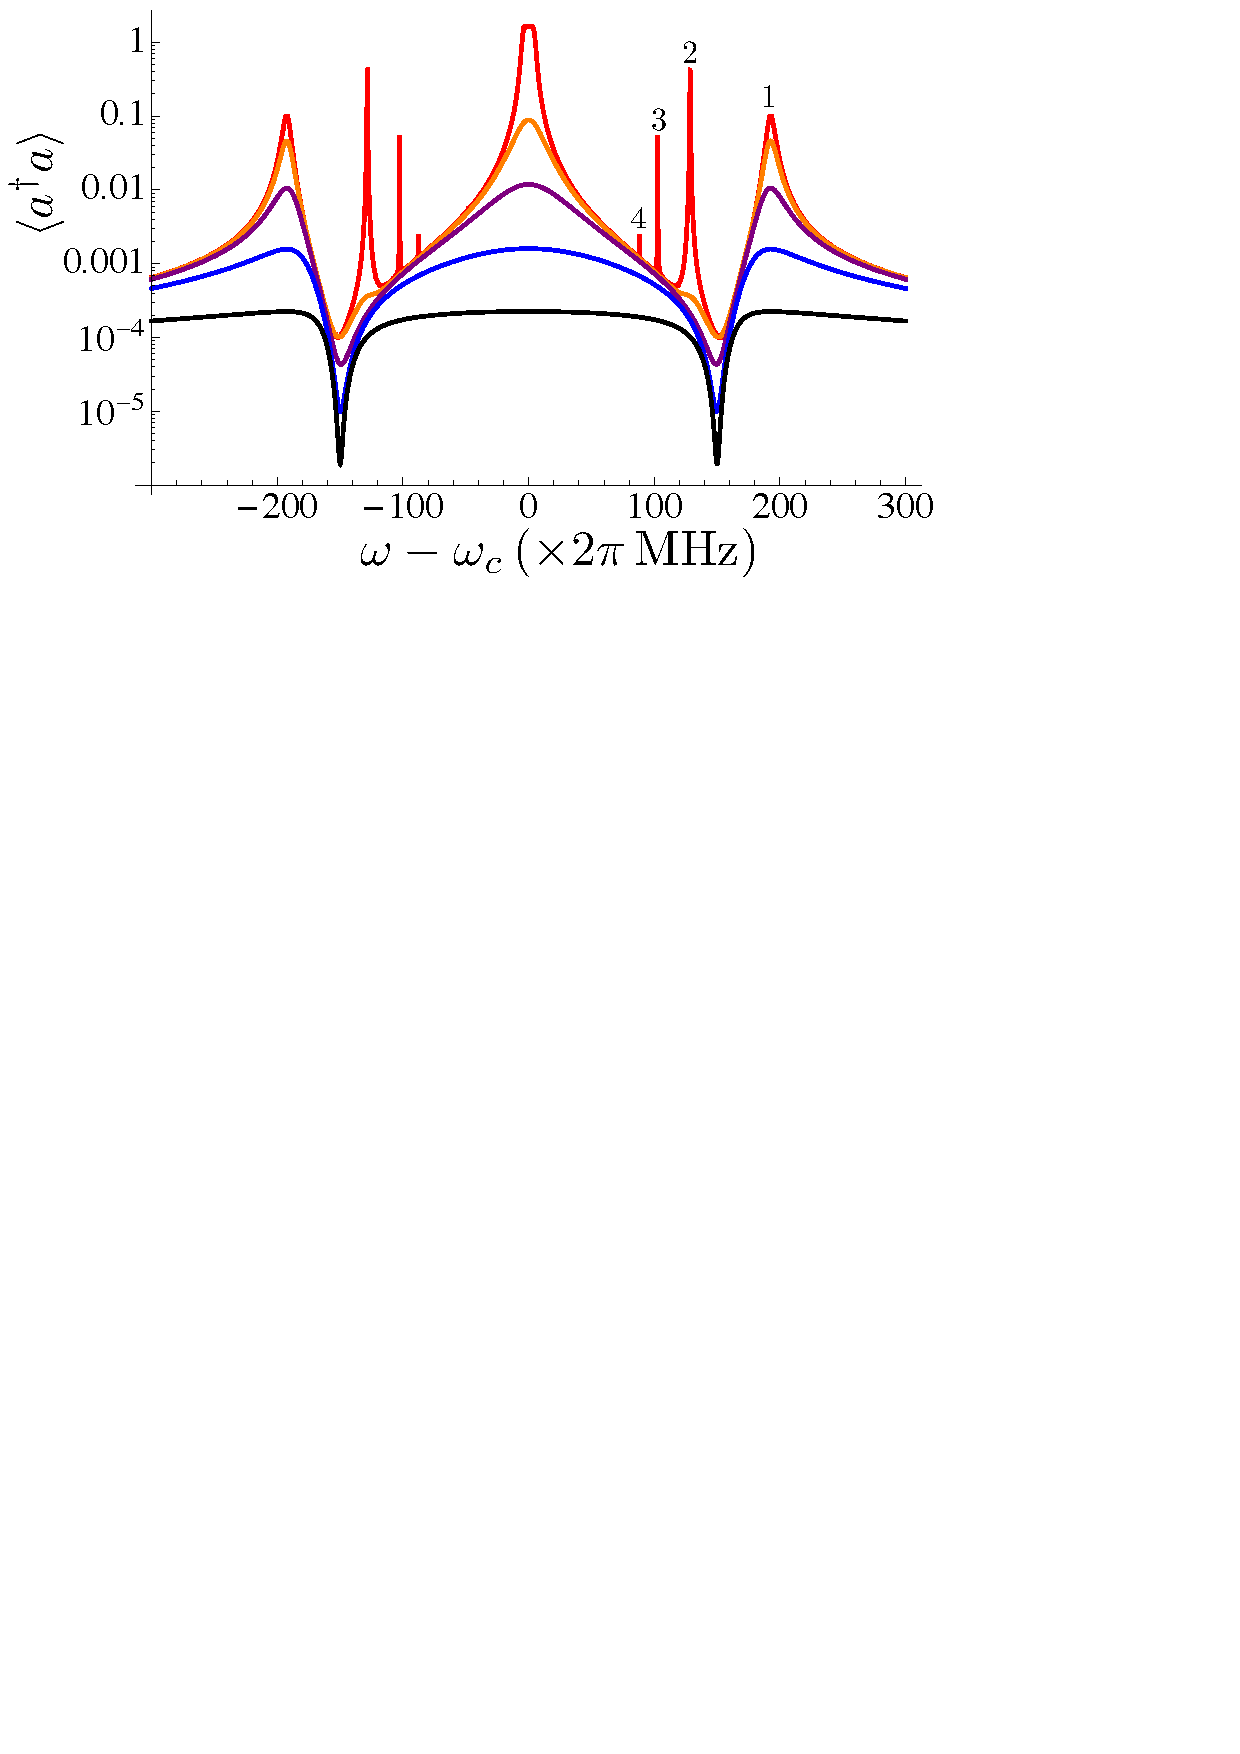
\includegraphics[width=0.75 \textwidth]{Images/chap5/aa_kappa.pdf}
    \caption[ $\mean{a^\dagger a}$ in function of $\omega-\omega_c$]{ Spectra of $\mean{a^\dagger a}$ in function of $\omega-\omega_c$ for the values in Tab.~\ref{tab-values}, $\Delta=150 \times 2\pi\,\mbox{MHz}$ and different values of $\kappa$ (in $2\pi$~MHz): 0 (Red); 20 (Orange); 55 (Purple); 150 (Blue); 400 (Black). The peaks are numbered in function of the order of the transitions at $\omega-\omega_c=\lambda_n/n$.}
    \label{fig-aa_kappa}
\end{figure}

First we study the transmission spectra, shown in Fig~\ref{fig-aa_kappa}, for different values of $\kappa$ and $\Delta=150 \times 2\pi\,\mbox{MHz}$. When the cavity decay rate is great, the $\mean{a^\dagger a}$ spectrum obtained is a typical one-photon absorption spectrum, with dips located at the two atomic frequencies, $\omega_c \pm \Delta$, which is similar to the case of two atoms in a vacuum. There is no other visible structure for cavities of such low quality.

When the cavity quality increases, peaks progressively start to appear at the frequencies of all the allowed transitions. In a perfect cavity, the amplitude of the peaks becomes very important and we observe several peaks numbered on the plot, corresponding to the $n$-photon processes $\ket 0 \rightarrow \ket{n,\pm}$ at $\omega-\omega_c=\lambda_n/n$ for $n=1,2,3,4$. We also note the amplitude of the central peak at $\omega=\omega_c$, which corresponds to all the consecutive one-photon transitions $\ket 0 \rightarrow \ket{1,0}\rightarrow \cdots \rightarrow \ket{n,0_{a,b}}$.


%\begin{figure}
%\center
%\includegraphics[width=0.75 \textwidth]{Images/chap5/aaaa_kappa.pdf}
%\caption{ Spectra of $\mean{(a^\dagger)^2 a^2}$ in function of $\omega-\omega_c$ for the values in Tab.~\ref{tab-values}, $\Delta=150$ and different values of $\kappa$: 0 (Red); 20 (Orange); 55 (Purple); 150 (Blue); 400 (Black).  }
%\label{fig-aa_kappa}
%\end{figure}

%In the $\langle (a^\dagger)^2 a^2 \rangle$ spectrum, the situation is similar, going from an absorption peak at the atomic frequencies to the transition peaks due to the coupling with the cavity and the dressed state structure.

\begin{figure}
    \center
    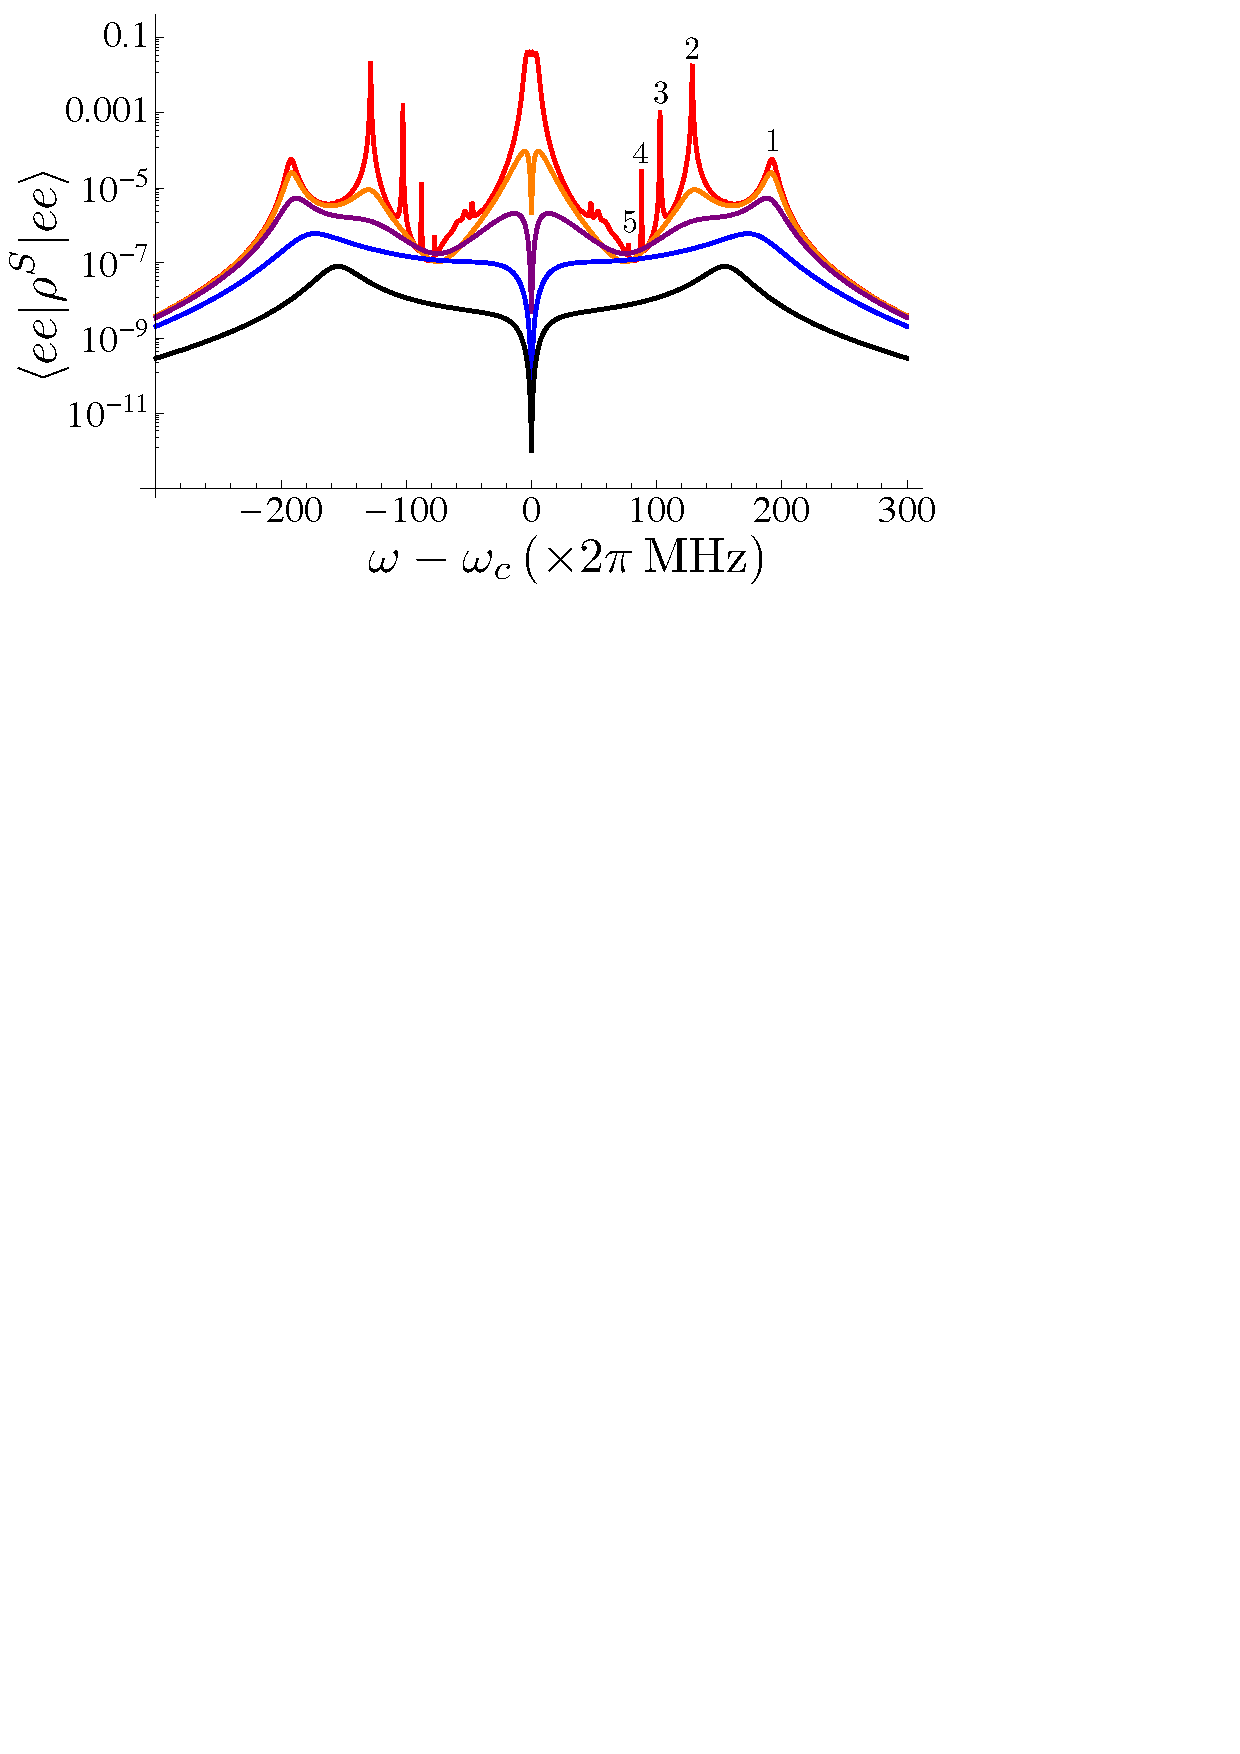
\includegraphics[width=0.75 \textwidth]{Images/chap5/ee_kappa.pdf}
    \caption[ $\prodsc{ee}{\rho^S}{ee}$ in function of $\omega-\omega_c$]{ Spectra of $\prodsc{ee}{\rho^S}{ee}$ in function of $\omega-\omega_c$ for the values in Tab.~\ref{tab-values}, $\Delta=150 \times 2\pi\,\mbox{MHz}$ and different values of $\kappa$ (in $2\pi$~MHz): 0 (Red); 20 (Orange); 55 (Purple); 150 (Blue); 400 (Black). The peaks are numbered in function of the order of the transitions at $\omega-\omega_c=\lambda_n/n$. }
    \label{fig-ee_kappa}
\end{figure}

Let us now study another aspect of the system and measure the populations of the excited states $\ket{e_1}$ and $\ket{ee}$ in the steady state $\rho^S$ in function of the laser frequency $\omega$. The quantities $\prodsc{e_1}{\rho^S}{e_1}$ and $\prodsc{ee}{\rho^S}{ee}$ will be considered, where the traces over the subsystems of no direct interest, namely the photon field and the second atom, is implied. Those atomic populations can be measured in circuit-QED~\cite{Fil09}.

In Fig.~\ref{fig-ee_kappa} we plotted the spectrum of $\prodsc{ee}{\rho^S}{ee}$. For a lossless cavity (in red) we observe transition peaks corresponding to the $n$-photon processes $\ket 0 \rightarrow \ket{n,\pm}$ at $\omega-\omega_c=\lambda_n/n$ for $n$ up to 5, all numbered on the figure. Between the peak number five and the central peak we can distinguish a few small peaks. It can be shown that those peaks correspond to the transitions $\ket{1,\pm} \rightarrow \ket{n,\pm}$ with $n\ge2$, which happen at the frequencies $\omega=\omega_c \pm (\lambda_n-\lambda_1)/(n-1)$. That second series of excitations is made possible thanks to the strength of the laser which populates the $\ket{1,\pm}$ states even away from resonance.

For cavities of lesser quality, the peaks quickly start to fade away. For the worst cavity we considered (in black), we see the apparition of two peaks, who are actually centered on the atomic frequencies $\omega-\omega_c = \pm 150 \times 2\pi\,\mbox{MHz}$, a behavior we would expect from the ionization spectrum of two atoms in free space, as in Fig.~\ref{fig-free}. We also note the apparition of a dip at the frequency $\omega=\omega_c$. We saw in Sec.~\ref{sec-free} that in free space the transition are $2\omega=\omega_1+\omega_2$ was prohibited by Fermi's golden rule, although that prohibition in the perturbation theory did not translate in the steady state behavior by an interference or a dip, but rather simply by an absence of peak. In our case, for a low quality cavity, the $\omega=\omega_c$ transition to the $\ket{ee}$ state is strictly prohibited unlike the photonic transitions shown in Fig.~\ref{fig-spec150}, even though they are both predicted to happen by perturbation theory. At this stage, we can only assume that this behavior is induced by the cavity decay mechanisms which are not considered in Fermi's golden rule and more calculations should be made in order to understand this phenomenon completely.

\begin{figure}
    \center
    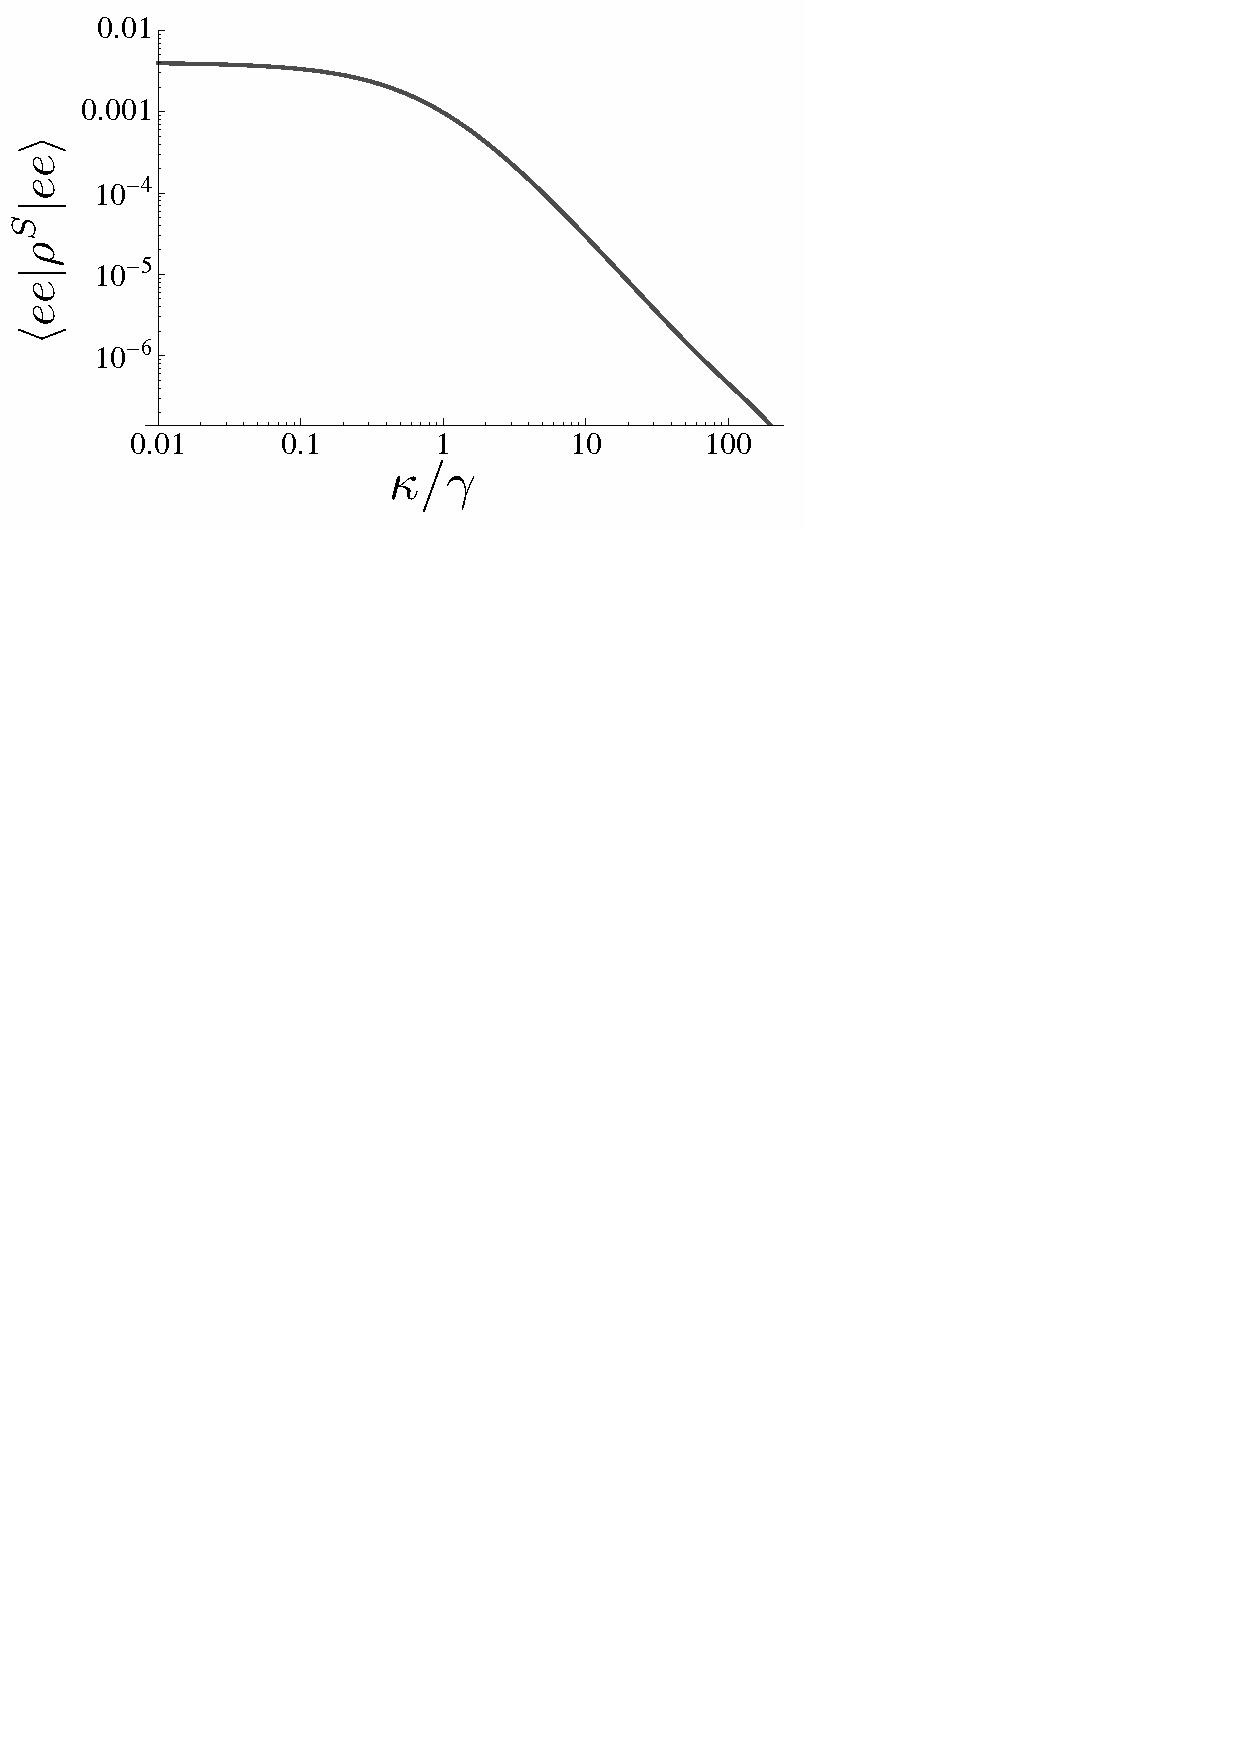
\includegraphics[width=0.65 \textwidth]{Images/chap5/kappa.pdf}
    \caption[$\prodsc{ee}{\rho^S}{ee}$ in function of $\kappa$]{ Spectrum of $\prodsc{ee}{\rho^S}{ee}$ in function of $\kappa$ for the values in Tab.~\ref{tab-values}, $\Delta=150 \times 2\pi\,\mbox{MHz}$ at the resonance $\omega=\omega_c+ \lambda_2/2$. For $\kappa\ll \gamma$ the population is saturated by the spontaneous emission, it then decreases following a power law as $\kappa$ grows beyond $\gamma$.}
    \label{fig-kappa}
\end{figure}

In Fig.~\ref{fig-kappa}, we study the diminution of the peak amplitude of $\prodsc{ee}{\rho^S}{ee}$ at the frequency $\omega=\omega_c + \lambda_2/2$ in function of $\kappa/\gamma$. Clearly, when $\kappa \ll \gamma$ the amplitude saturates, i.~e.~the population of the doubly excited atoms is limited by the spontaneous emission, but another regime is reached when $\kappa \gg \gamma$ where the amplitude is decreased following a power law. We therefore see that the best amplitudes are reached for the cavity decay rate smaller or of the order of the atomic decay rate.


\begin{figure}
    \center
    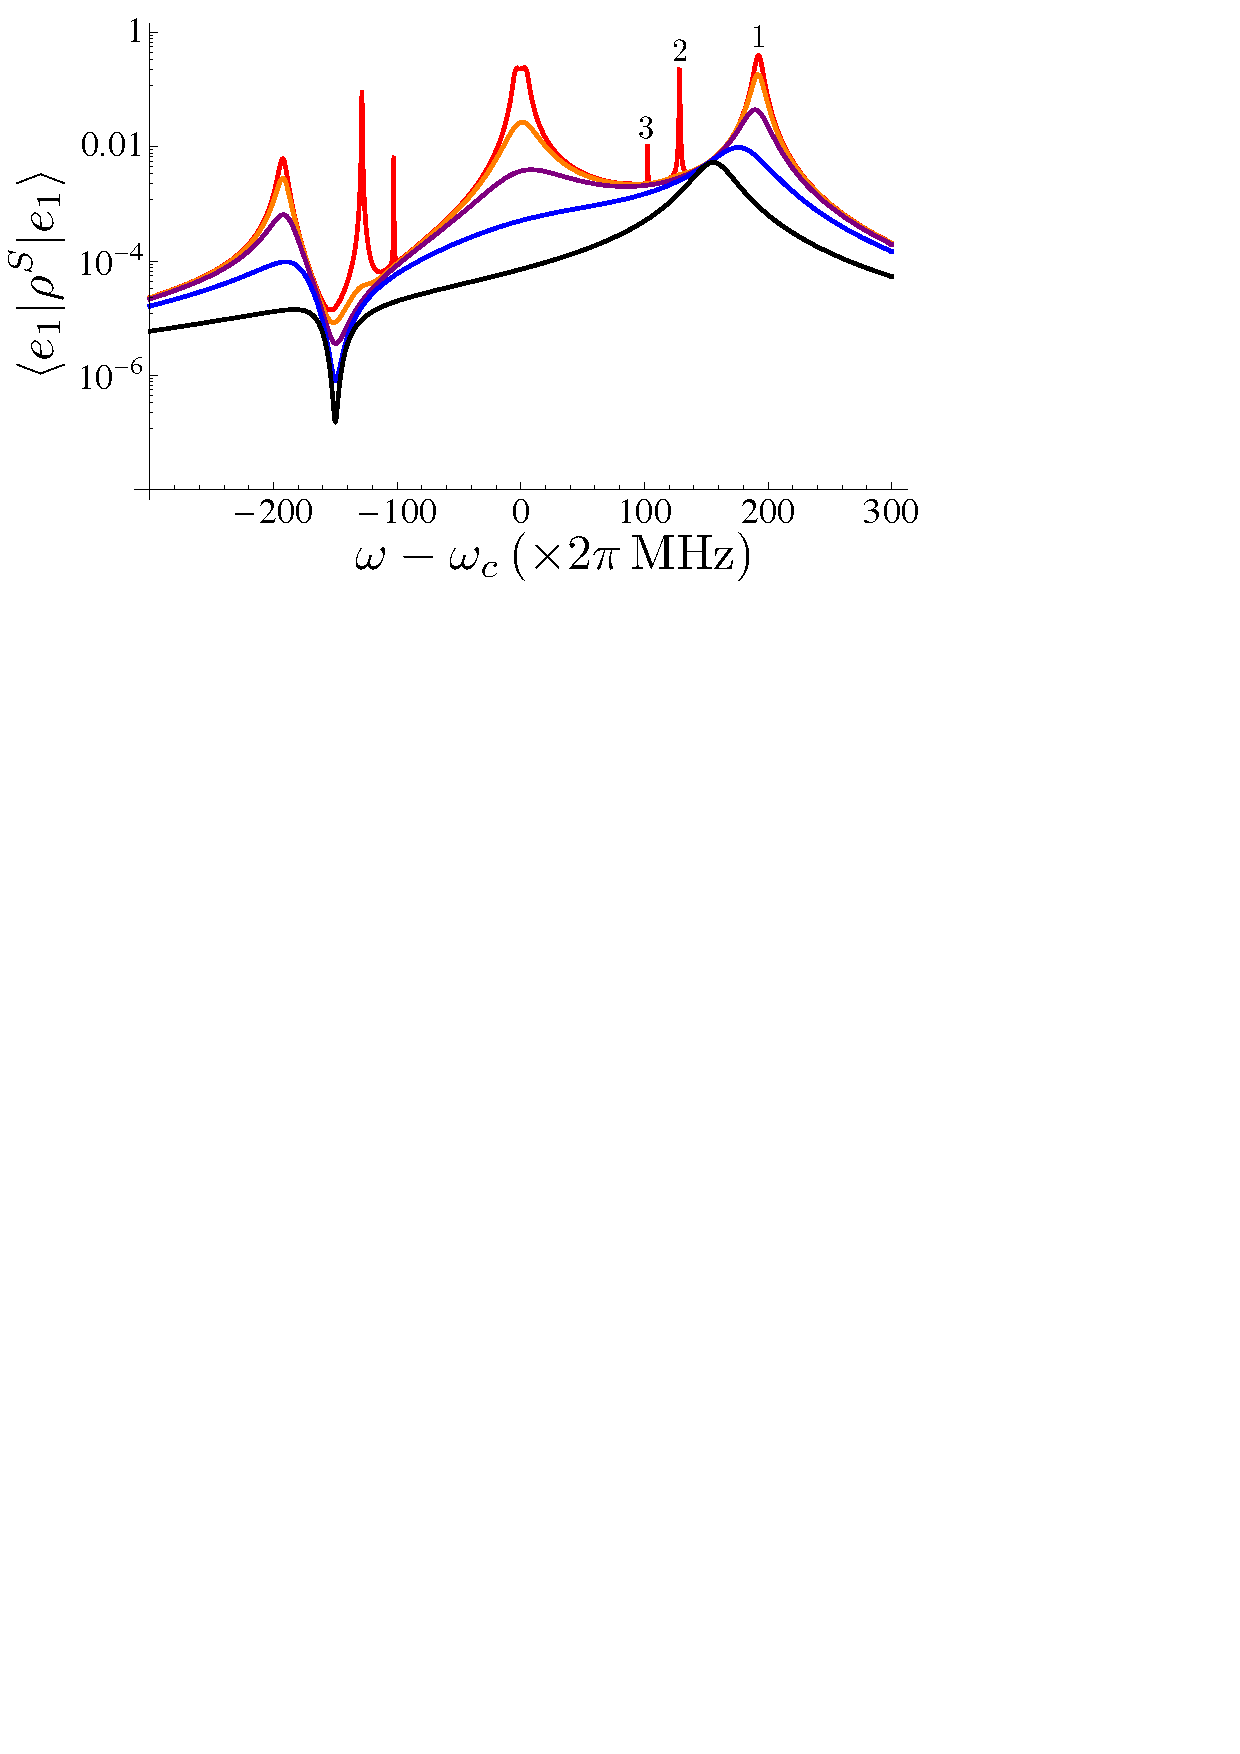
\includegraphics[width=0.75 \textwidth]{Images/chap5/eg_kappa.pdf}
    \caption[$\prodsc{e_1}{\rho^S}{e_1}$ in function of $\omega-\omega_c$]{ Spectra of $\prodsc{e_1}{\rho^S}{e_1}$ in function of $\omega-\omega_c$ for the values in Tab.~\ref{tab-values}, $\Delta=150 \times 2\pi\,\mbox{MHz}$ and different values of $\kappa$ (in $2\pi$~MHz): 0 (Red); 20 (Orange); 55 (Purple); 150 (Blue); 400 (Black). The peaks are numbered in function of the order of the transitions at $\omega-\omega_c=\lambda_n/n$. }
    \label{fig-eg_kappa}
\end{figure}


In Fig.~\ref{fig-eg_kappa}, we study the probability to observe only one of the atoms excited $\prodsc{e_1}{\rho^S}{e_1}$ in function of $\omega-\omega_c$. For a perfect cavity (in red), we observe once again transition peaks for the transitions $\ket 0 \rightarrow \ket{n,\pm}$ at $\omega-\omega_c=\lambda_n/n$ for $n$ up to 3, although the two higher order peaks are very thin and disappear completely for $\kappa=20\times 2\pi$~MHz which is easily understood since those are multi-photon processes measured on a single excitation spectrum, just as the two-photon peaks on $\mean{a^\dagger a}$ in Fig.~\ref{fig-spec150} was several orders of magnitude smaller than the one-photon peaks on $\mean{a^\dagger a}$.

For greater values of cavity decay rate, all the peaks begin to fade away until only one peak is left around the first internal atomic frequency at $\omega - \omega_c = 150 \times 2\pi\,\mbox{MHz}$, as we would expect from a spectrum of an atom in free space. What we would not expect from such a spectrum however is the dip that forms around the second atomic internal frequency  $\omega - \omega_c = -150 \times 2\pi\,\mbox{MHz}$. That new behavior is once again due to the cavity decay process in the system. Note that even though the presence of the $\ket{ee}$ state is strongly inhibited for finite $\kappa$ at the frequency $2\omega=\omega_1+\omega_2$, the presence of only one excited atom is not affected at all, which induces a strong blockade in the system, even if the two atoms do not interact directly with each other.

One interesting feature we also observe on the graph is that at the amplitude of the population of the $\prodsc{e_1}{\rho^S}{e_1}$ at the first atomic internal frequency $\omega - \omega_c = 150 \times 2\pi\,\mbox{MHz}$ seems to be completely independent from the value of $\kappa$. For a perfect cavity, there is no discernible peak at that location, but as the decay rate grows, the population stays the same while for all the other frequencies it weakens, which eventually yields a peak at the atomic frequency.

%\subsection{Three regimes of $P_{ee} (\kappa)$ } ?????


\section{General Atomic Frequency Spread}  \label{sec-phi}

In this section, we investigate the behavior of the system not being restrained by the constraint $\omega_1 + \omega_2 = 2 \omega_c$. For this general setup of the atomic frequencies, we are no longer able to diagonalize the unperturbed Hamiltonian or perturbation theory. We will rely purely on numerical considerations and analogies with the previous case.

We define the atomic frequencies to be
\bea
\omega_1 &=& \omega_c + \Delta + \phi, \\
\omega_2 &=& \omega_c - \Delta + \phi,
\eea
which yield every possible value of $\omega_1$ and $\omega_2$ when $\Delta$ and $\phi$ are allowed to vary. The particular case $\omega_1 + \omega_2 = 2 \omega_c$ is found when $\phi=0$.

\subsection{Eigenstates and Eigenvalues}

We showed in Sec.~\ref{sec-QEDMod} that the Hamiltonian $H$ always commutes with the global excitation number operator $\hat n$ without making any assumptions on the atomic frequencies. This means that $H$ keeps its block diagonal form described earlier, however we were unable to diagonalize the different blocks with general atomic internal frequencies. Although the analytical form of the eigenvalues and eigenstates are not generally known, except for the ground state $\ket 0$, we may still numerically identify them. We keep the notation previously used and call the $n=1$ excited states $\ket{1,0}, \ket{1,\pm}$ and the $n$ excited states $\ket{n,0_{a,b}}, \ket{n,\pm}$ with the respective eigenvalues 0, $\hbar\omega_c+\hbar\lambda^{(1,0)}$, $\hbar\omega_c+\hbar\lambda^{(1,\pm)}$, $n\hbar \omega_c+\hbar\lambda^{(n,0_{a,b})}$ and $n\hbar \omega_c+\hbar\lambda^{(n,\pm)}$. Although we do not now the analytical form of these eigenvalues, we can identify them from the values they have for $\phi=0$.

\begin{figure}
    \center
    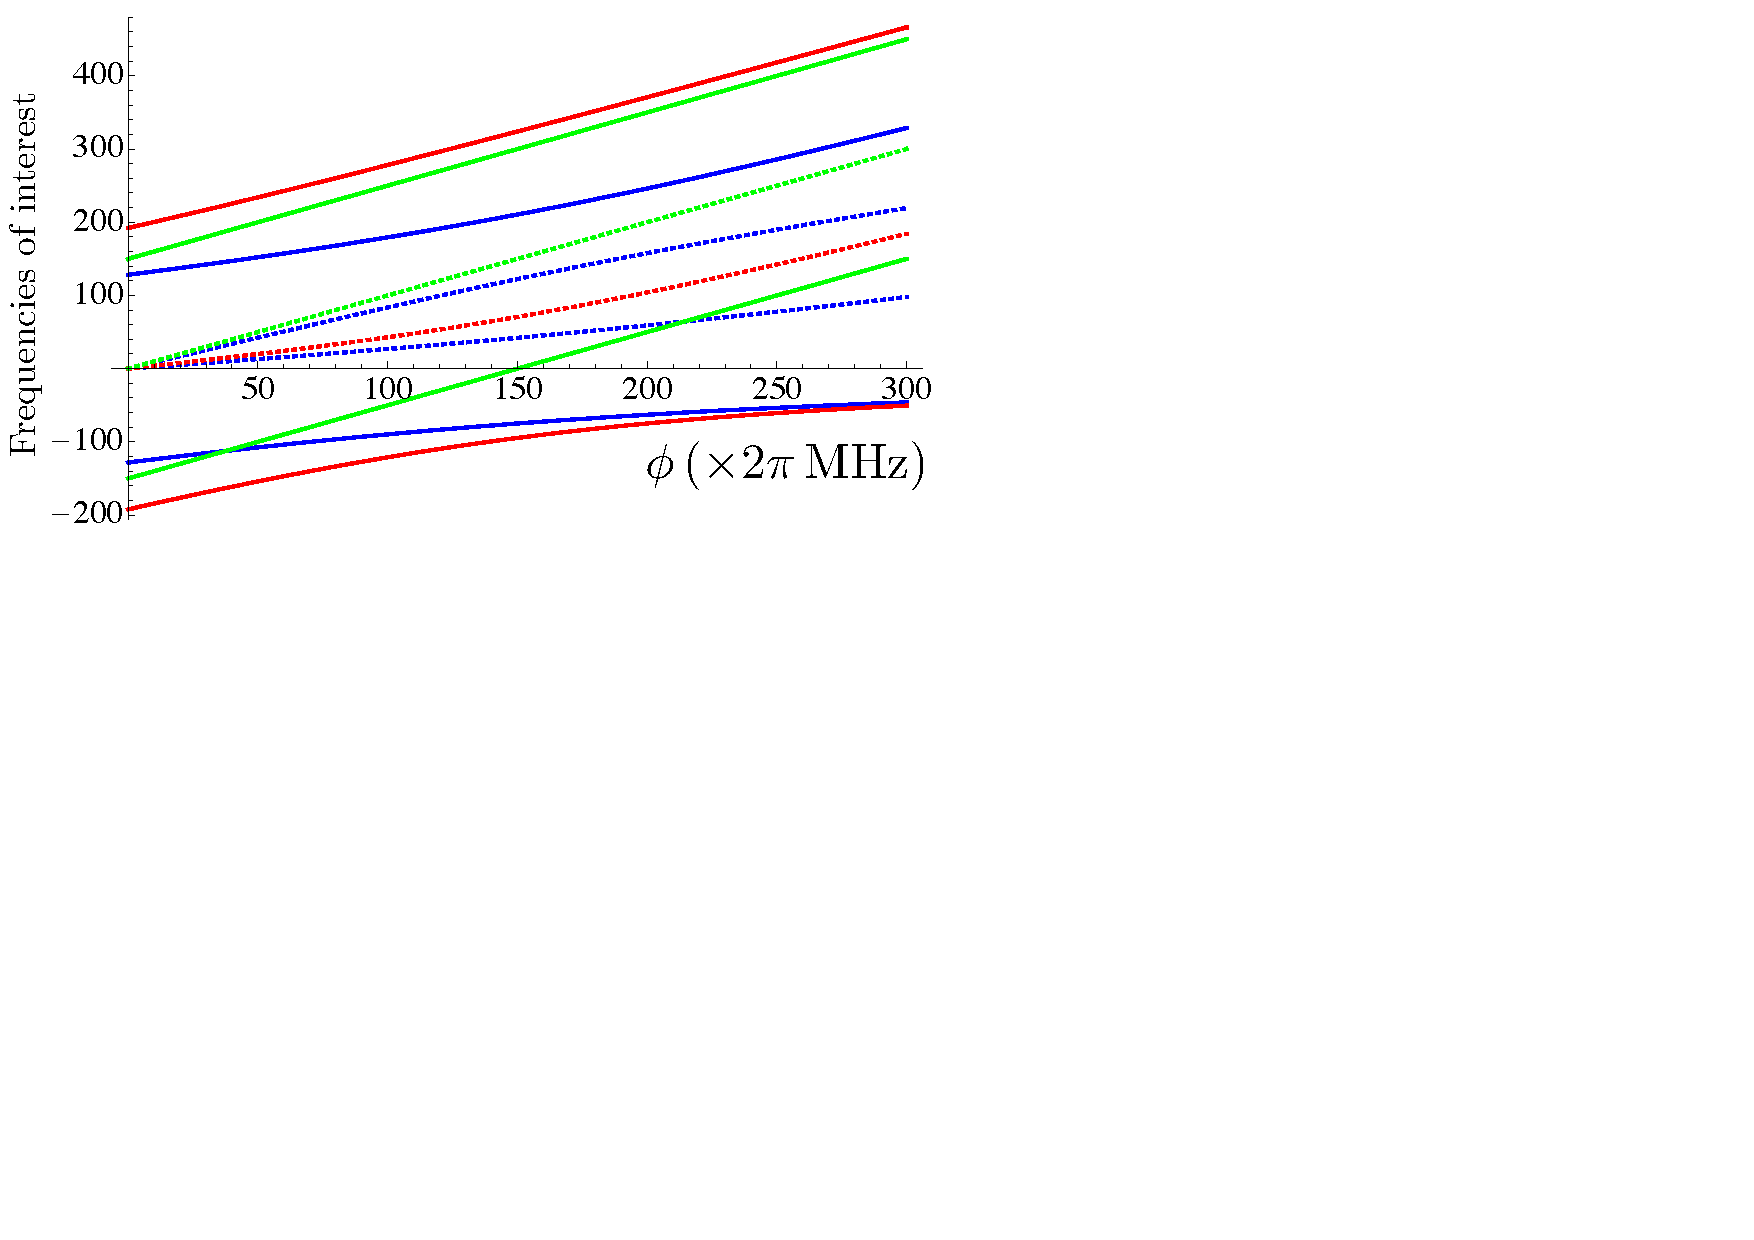
\includegraphics[width=0.75 \textwidth]{Images/chap5/transitions.pdf}
    \caption[Numerical values of $\lambda^{(1,0)}$]{Numerical values of $\lambda^{(1,0)}$ (red, dotted), $\lambda^{(1,\pm)}$ (red), $\lambda^{(2,0_{a,b})}/2$ (blue, dotted) and $\lambda^{(2,\pm)}/2$ (red) as well as $\omega_1$, $\omega_2$ (green) and $(\omega_1+\omega_2)/2$ (green, dotted) in function of $\phi$ for $\alpha = 85\times 2\pi\,\mbox{MHz}, \Delta = 150 \times 2\pi\,\mbox{MHz}$. The red and blue lines represent the values of $\omega-\omega_c$ a which one and two-photon transitions are expected and the green lines the values we might expect dips for different quantities. The dotted lines are  transition values that are degenerate when $\Delta=0$.}
    \label{fig-trans}
\end{figure}

In Fig.~\ref{fig-trans}, we show the numerical values of $\lambda^{(1,0)}$, $\lambda^{(1,\pm)}$, $\lambda^{(2,0_{a,b})}/2$ and $\lambda^{(2,\pm)}/2$ as well as $\omega_1$, $\omega_2$ and $(\omega_1+\omega_2)/2$ in function of $\phi$ for $\Delta=150\times 2\pi\,\mbox{MHz}$. We identify which eigenvalue is which from the initial values at $\phi=0$, with some uncertainty about $\lambda^{(2,0_{a})}$ and $\lambda^{(2,0_{b})}$ which are degenerate for $\phi=0$. We will shortly solve this problem.

We chose for the next numerical calculations to settle on the numerical parameter  $\phi=130 \times 2\pi\,\mbox{MHz}$ which spreads as evenly as possible all the numerical values plotted in an attempt to separate the possible peaks and dips as well as possible. We used in the previous calculations a high laser strength $\epsilon=6 \times 2\pi\,\mbox{MHz}$ in order to maximize the visibility of the two-photon processes in the spectra. Unfortunately, using a high laser power also broadens the peaks and as we now  investigate a more general case with a more complex structure, we will use the smaller value $\epsilon= 2\pi\,\mbox{MHz}$ to separate the peaks more effectively.

In the particular case  of two identical atoms, i.~e.~when $\Delta=0$, we can partially diagonalize the blocks of the unperturbed Hamiltonian and find a few eigenstates. These eigenvectors are
\begin{align}
    \ket{1,0}   & = \frac{1}{\sqrt 2} \left( \ket{0,eg}  - \ket{0,ge} \right),                                                                                \\
    \ket{1,\pm} & = \frac{1}{\sqrt{2\alpha^2 + (\lambda^{(1,\pm)})^2 }} \left( \alpha \ket{0,eg} + \alpha \ket{0,ge} - \lambda^{(1,\pm)} \ket{1,gg} \right) , \\
    \ket{2,0_b} & = \frac{1}{\sqrt 2} \left( \ket{1,eg}  - \ket{1,ge} \right),
\end{align}
and the other ones were not found. We chose to call the last state $\ket{2,0_b}$ rather than $\ket{2,0_a}$ since it is actually the same as the case $\phi=0$. Note that $\ket{1,0}$ and $\ket{2,0_b}$ are again antisymmetrical under the permutation of the two atoms and are again decoupled from the other states. We can also calculate the respective eigenvalues to the eigenstates and we find that $\lambda^{(1,0)} = \Delta$, $\lambda^{(1,\pm)} =( \Delta \pm \sqrt{8\alpha^2+\Delta^2})/2$ and $\lambda^{(2,0_b)}= \Delta$. Numerically, starting from that situation, we checked that value of $\lambda^{(2,0_b)}$ is always smaller than $\lambda^{(2,0_a)}$ for other values of $\Delta$ and $\phi$ and the uncertainty about their respective denomination is lifted.

We can calculate the few off-diagonal terms coming from the perturbation $W$ linking those eigenstates, which are expressed, in the unperturbed Hamiltonian eigenstates basis, as
\bea
\prodsc{0}{W}{1,0} &=& 0 ,\\
\prodsc{0}{W}{1,\pm} &=&   -i \,\frac{\lambda^{(1,\pm)}}{{\sqrt{2\alpha^2 + (\lambda^{(1,\pm)})^2 }}} \, \epsilon, \\
\prodsc{1,0}{W}{2,0_b} &=& - i \epsilon,\\
\prodsc{1,\pm}{W}{2,0_b} &=& 0,
\eea
which indicates that, because of their antisymmetry, the $\ket{1,0}$ and $\ket{2,0_b}$ states do not get populated by the perturbation by either one or two-photon processes.

\subsubsection{Atomic, one and two-photon Spectroscopy}

\begin{figure}
    \center
    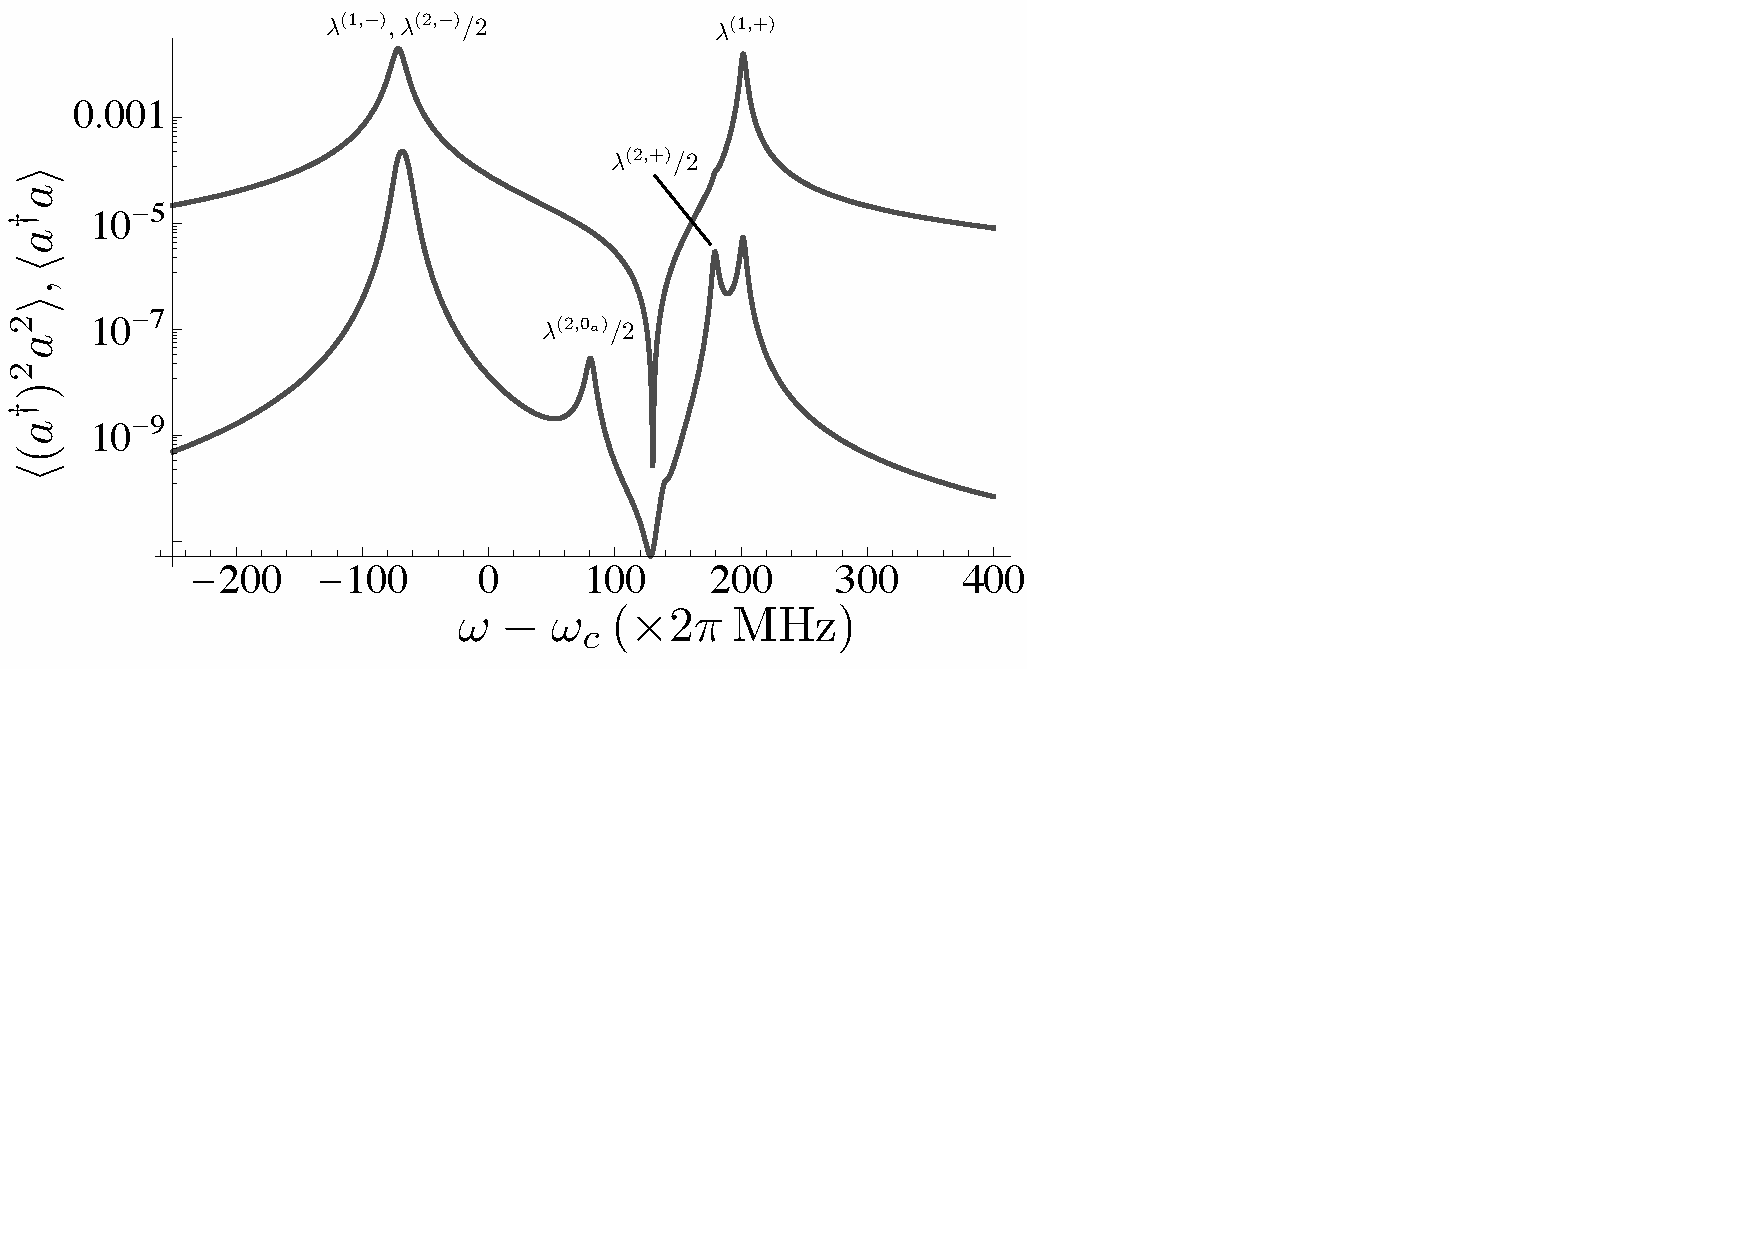
\includegraphics[width=0.74 \textwidth]{Images/chap5/aa_cool_0.pdf}
    \caption[$\langle a^\dagger a \rangle$ and $\langle (a^\dagger)^2 a^2 \rangle$ in function of $\omega-\omega_c$]{ Spectra of $\langle a^\dagger a \rangle$ (top) and $\langle (a^\dagger)^2 a^2 \rangle$ (bottom) in function of $\omega-\omega_c$ for the values in Tab.~\ref{tab-values}, $\epsilon=2\pi\,\mbox{MHz}$, $\Delta=0$ and $\phi=130 \times 2\pi\,\mbox{MHz}$. We find two  peaks at $\omega-\omega_c=\lambda^{(1,\pm)}$ corresponding to one-photon transitions and three peaks at $\omega-\omega_c = \lambda^{(2,\pm)}/2$ and $\lambda^{(2,0_a)}/2$ corresponding to the two-photon transitions. No trace of transitions involving the states $\ket{1,0}$ or $\ket{n,0_b}$. We also find a dip at the atomic frequencies $\omega_1=\omega_2=\omega_c+ \Delta$.}
    \label{fig-aa_cool_0}
\end{figure}

Let us now study the different spectra of the general steady state case. We show in Fig.~\ref{fig-aa_cool_0} the $\langle a^\dagger a \rangle$ and $\langle (a^\dagger)^2 a^2 \rangle$ spectra of the particular case $\Delta=0$. As we expected, there is no peak at  $\omega = \omega_c$, on the contrary we find there a strong dip in the populations at the atomic frequencies $\omega_1=\omega_2=\omega_c$, due once again to the cavity decay process. We find two-photon peaks in the $\langle (a^\dagger)^2 a^2 \rangle$ spectrum (and a beginning of a three-photon peak around $\omega-\omega_c \simeq 140\times 2\pi\,\mbox{MHz}$), although the peak at $\lambda^{(2,-)}/2$ happens to be very close to the one-photon peak at $\lambda^{(1,-)}$ and those two are not resolved but yield a peak of consequently greater amplitude than the peak at $\lambda^{(2,+)}/2$.

\begin{figure}
    \center
    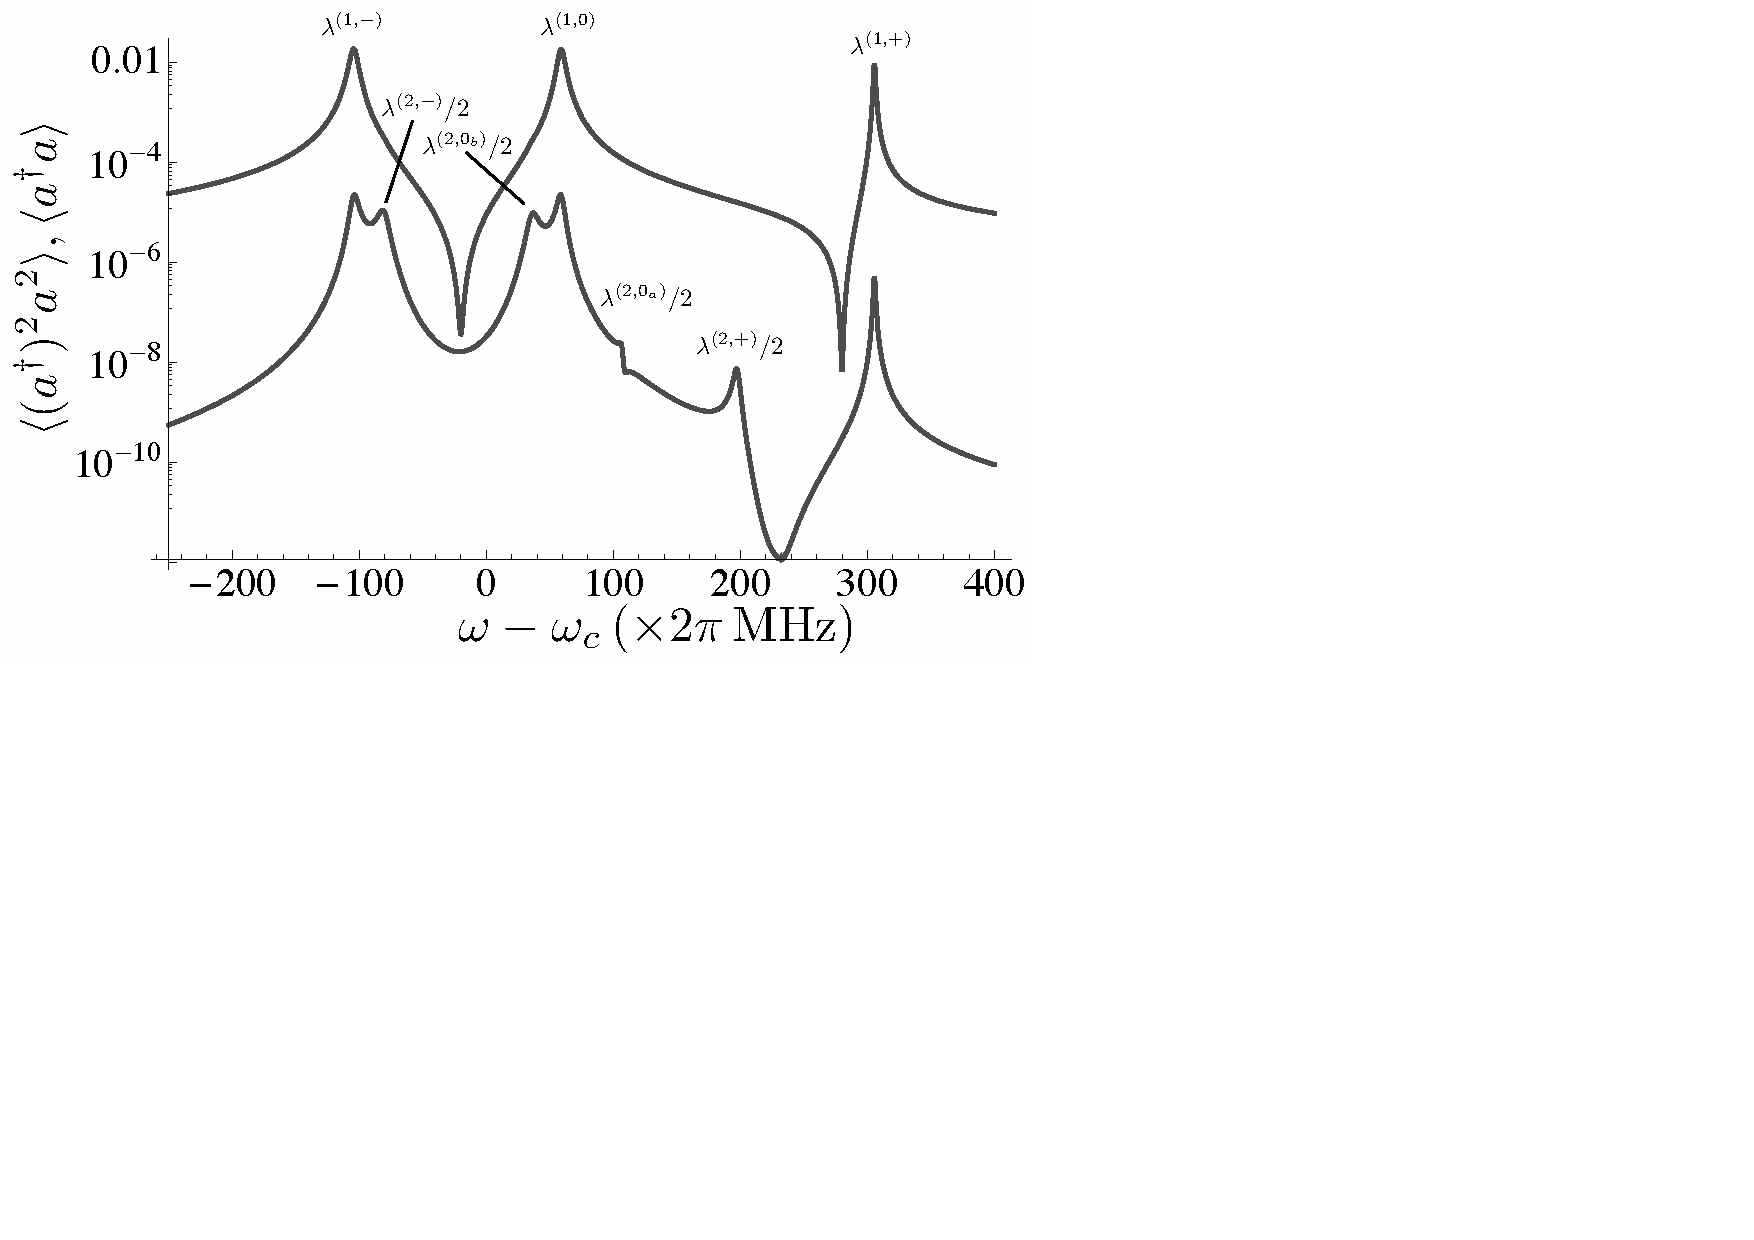
\includegraphics[width=0.74 \textwidth]{Images/chap5/aa_cool_150.pdf}
    \caption[$\langle a^\dagger a \rangle$ and $\langle (a^\dagger)^2 a^2 \rangle$ in function of $\omega-\omega_c$ ]{Spectra of $\langle a^\dagger a \rangle$ (top) and $\langle (a^\dagger)^2 a^2 \rangle$ (bottom) in function of $\omega-\omega_c$ for the values in Tab.~\ref{tab-values}, $\epsilon= 2\pi\,\mbox{MHz}$, $\Delta=150 \times 2\pi\,\mbox{MHz}$ and $\phi=130\times 2\pi\,\mbox{MHz}$.  We find three peaks at $\omega-\omega_c=\lambda^{(1,\pm)}$ and $\lambda^{(1,0)}$ corresponding to one-photon transitions and four peaks at $\omega-\omega_c = \lambda^{(2,\pm)}/2$ and $\lambda^{(2,0_{a,b})}/2$ corresponding to two-photon transitions. We also find two dips at the atomic frequencies $\omega-\omega_c=280 \times 2\pi\,\mbox{MHz}$ and $\omega-\omega_c=-20 \times 2\pi\,\mbox{MHz}$.}
    \label{fig-aa_cool_150}
\end{figure}

Let us now investigate the more general case $\Delta=150 \times 2\pi\,\mbox{MHz}$ and $\phi = 130\times 2\pi\,\mbox{MHz}$, of which we plotted the $\langle a^\dagger a \rangle$ and $\langle (a^\dagger)^2 a^2 \rangle$ spectra in Fig.~\ref{fig-aa_cool_150}. We count three one-photon peaks, all associated with one $n=1$ eigenvalue and four two-photon peaks, again associated with the four $n=2$ eigenvalues. We find two important dips in $\langle a^\dagger a \rangle$ located at the two atomic frequencies $\omega-\omega_c=280 \times 2\pi\,\mbox{MHz}$ and $\omega-\omega_c=-20 \times 2\pi\,\mbox{MHz}$ which is a cavity decay related process. In the $\langle (a^\dagger)^2 a^2 \rangle$ spectrum, the same dips are not visible, but we see the apparition of a new one around $\omega-\omega_c \simeq 225 \times 2\pi\,\mbox{MHz}$ that does not seem to correspond to any particular value we used up until now.

\begin{figure}
    \center
    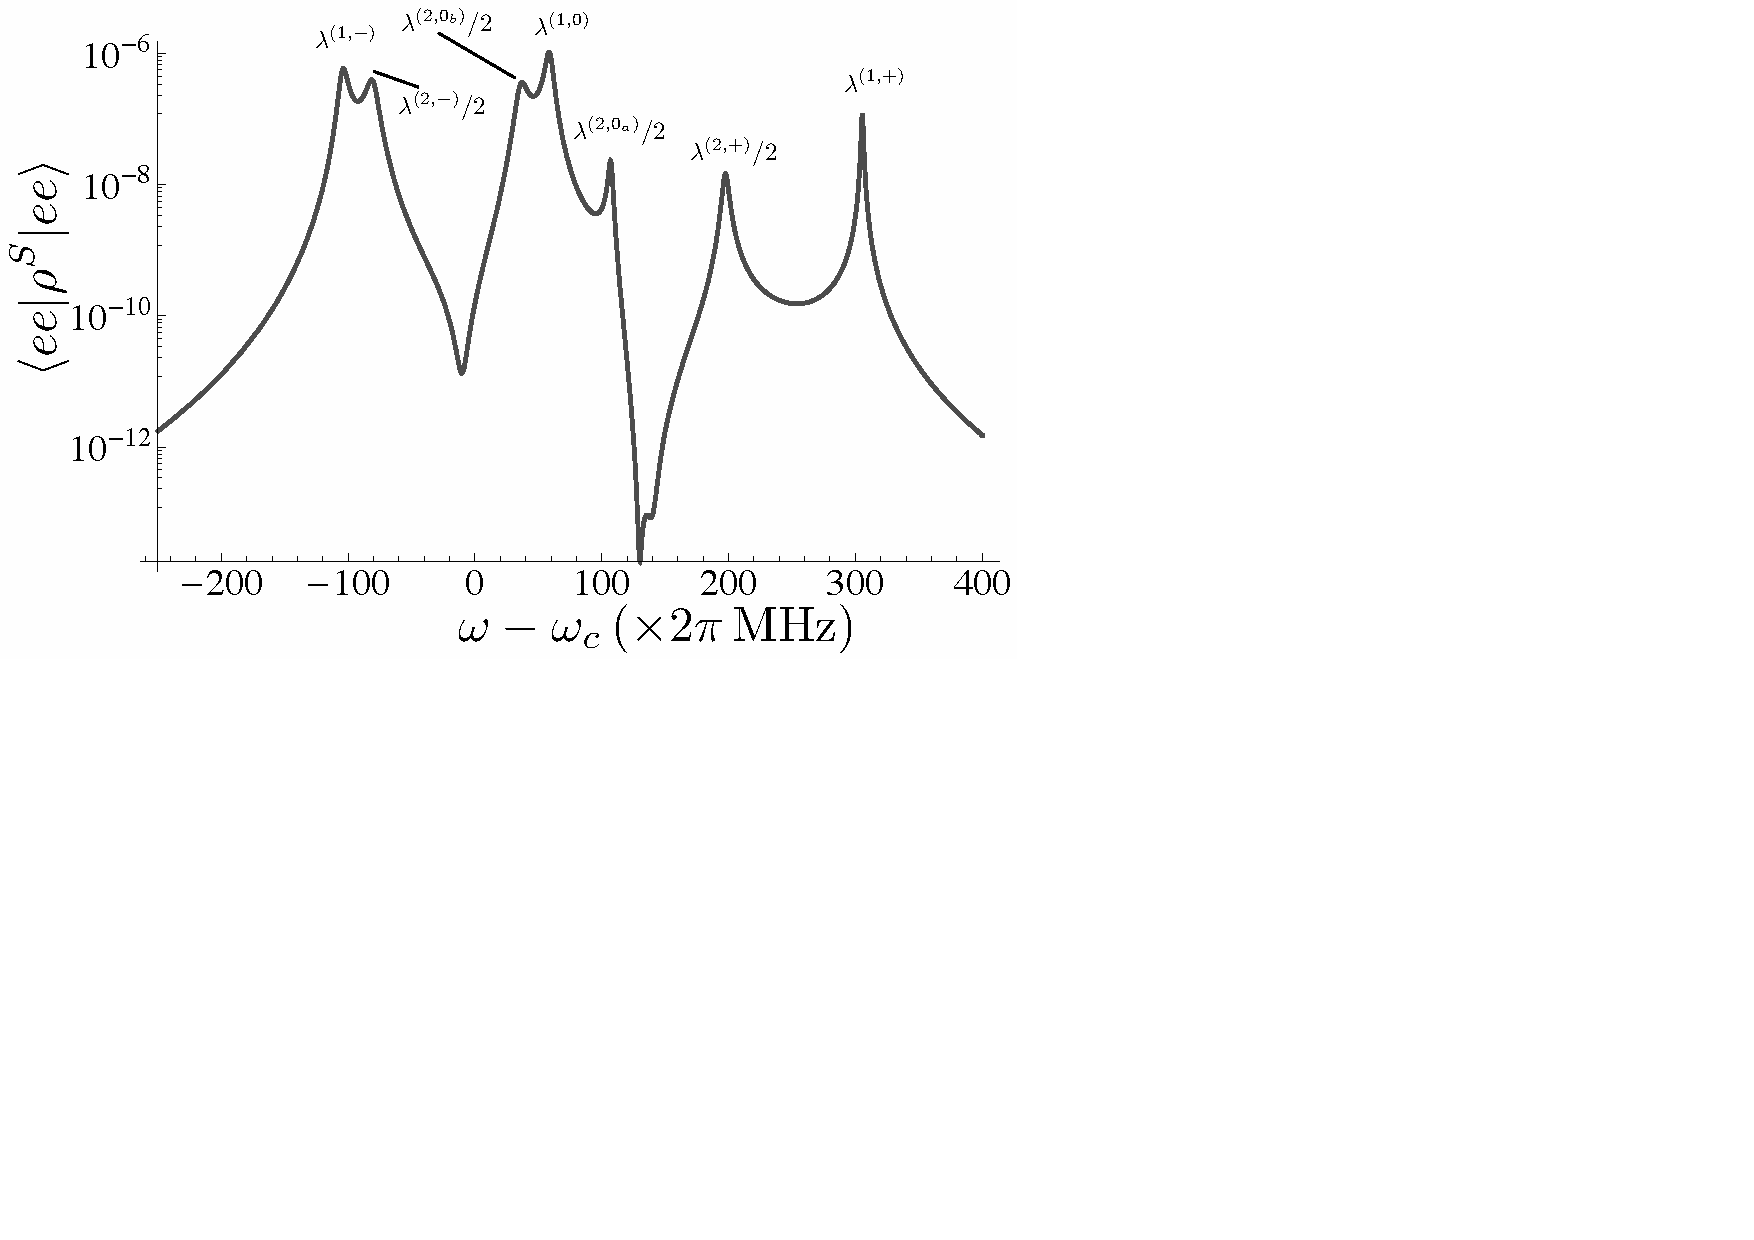
\includegraphics[width=0.75 \textwidth]{Images/chap5/ee_cool.pdf}
    \caption[$\prodsc{ee}{\rho^S}{ee}$ in function of $\omega-\omega_c$]{Spectrum of $\prodsc{ee}{\rho^S}{ee}$ in function of $\omega-\omega_c$ for the values in Tab.~\ref{tab-values}, $\epsilon= 2\pi\,\mbox{MHz}$, $\Delta=150 \times 2\pi\,\mbox{MHz}$ and $\phi=130\times 2\pi\,\mbox{MHz}$. We find three peaks at $\omega-\omega_c=\lambda^{(1,\pm)}$ and $\lambda^{(1,0)}$ corresponding to all possible one-photon transitions and four peaks at $\omega-\omega_c = \lambda^{(2,\pm)}/2$ and $\lambda^{(2,0_{a,b})}/2$ corresponding to all possible two-photon transitions. We also count three dips, two small ones at the atomic frequencies and an important one at the mean frequency $\omega-\omega_c = 130 \times 2\pi\,\mbox{MHz}$.}
    \label{fig-ee_cool}
\end{figure}

In Fig.~\ref{fig-ee_cool} we plotted the spectrum of $\prodsc{ee}{\rho^S}{ee}$ in function of $\omega-\omega_c$ also for $\Delta=150\times 2\pi\,\mbox{MHz}$ and $\phi = 130\times 2\pi\,\mbox{MHz}$. We count seven peaks, three associated one-photon processes and four associated two-photon processes. This is the most general case where there is no interference between the different excitation paths that lead to an inhibition of a peak. We also count three different dips, two of them of weak amplitude located at the atomic frequencies $\omega-\omega_c=280\times 2\pi\,\mbox{MHz}$ and $\omega-\omega_c=-20\times 2\pi\,\mbox{MHz}$, and a very strong one located at the half-sum of the frequencies $\omega - \omega_c = 130\times 2\pi\,\mbox{MHz}$, once again linked with the cavity decay process.

\subsection{Cavity Induced Transparency}

Let us investigate another property of two atoms in a cavity. We showed in Eq.~(\ref{eq-QEDempty}) the spectrum of the mean number of photon $\mean{a^\dagger a}$ in an empty cavity. Using the same formalism we will derive the analytical expression of $\mean{a^\dagger a}$ in an empty cavity and show that
\[\mean{(a^\dagger)^2 a^2}=(\mean{a^\dagger a})^2.\]

For that, we use Eq.~(\ref{eq-dAdt}) with $A=(a^\dagger)^2 a^2$ and we calculate
\begin{align}
     & [A, a^\dagger a]=0, \;\; [A, a^\dagger ] = 2a^\dagger a^\dagger a, \;\; [A, a]= -2 a^\dagger aa, \\
     & Aa^\dagger a  - 2 a^\dagger A a + a^\dagger a A= 2 a^\dagger a^\dagger aa  ,
\end{align}
where we used the basic commutation relations $[a,a^\dagger]=1$ to find the final results. We find
\[ \frac{d}{dt} \mean{(a^\dagger)^2 a^2} = 2\epsilon( \mean{a^\dagger a^\dagger a}+ \mean{a^\dagger aa})  - 4 \kappa \mean{(a^\dagger)^2 a^2},\]
and we have to calculate the time variation of $ \mean{a^\dagger a^\dagger a}$.  Let us pose $B= a^\dagger a^\dagger a$ and we have
\begin{align}
     & [B, a^\dagger a]= - a^\dagger a^\dagger  a, \;\; [B, a^\dagger ] =a^\dagger a^\dagger ,\;\; [B, a]= -2a^\dagger a, \\
     & Ba^\dagger a  - 2 a^\dagger B a + a^\dagger a B=3 a^\dagger a^\dagger a.
\end{align}
We have
\[ \frac{d}{dt} \mean{a^\dagger a^\dagger a} = \left( i(\omega_c-\omega) - 3 \kappa \right)  \mean{a^\dagger a^\dagger a}+\epsilon( \mean{a^\dagger a^\dagger} +2 \mean{a^\dagger a}),\]
and with $\frac{d}{dt} \mean{a^\dagger a a}$ its complex conjugate. There is one more the time variation to calculate. With $C=a^2$ we have
\begin{align}
     & [C, a^\dagger a]= 2aa , \;\; [C, a^\dagger ] = 2a , \;\; [C, a]= 0, \\
     & Ca^\dagger a  - 2 a^\dagger C a + a^\dagger a C= 2aa,
\end{align}
and we have
\[ \frac{d}{dt} \mean{a^2} = 2\left( -i(\omega_c-\omega) - \kappa \right)  \mean{a^2}+2 \epsilon \mean{a}.\]
and with $\frac{d}{dt} \mean{(a^\dagger)^2}$ its complex conjugate.

Globally, in the steady state, we have
\bea
\mean{a}&=& \frac{\epsilon}{\kappa+i(\omega_c-\omega)} ,\\
\mean{a^\dagger a}&= & \frac{\epsilon^2}{\kappa^2+(\omega_c-\omega)^2}= \mean{a^\dagger}\mean{a} ,\\
\mean{a^2}&=& \frac{\epsilon \mean{a}}{\kappa+i(\omega_c-\omega)}= \mean{a}^2 ,\\
\mean{a^\dagger a^\dagger a} &=& \frac{\epsilon( \mean{a^\dagger a^\dagger} +2 \mean{a^\dagger a})}{ 3 \kappa - i(\omega_c-\omega)}=  \epsilon \mean{a^\dagger} \frac{ \mean{a^\dagger} +2 \mean{a}}{ 3 \kappa - i(\omega_c-\omega)} = \mean{a^\dagger} \mean{a^\dagger a}, \\
\mean{(a^\dagger)^2 a^2} &=& \frac{\epsilon}{2\kappa}( \mean{a^\dagger a^\dagger a}+ \mean{a^\dagger aa}) =  \frac{\epsilon}{2\kappa} \mean{a^\dagger a} (\mean{a^\dagger}+\mean{a}) = \mean{a^\dagger a}^2,
\eea
and we have the desired result.

\begin{figure}
    \center
    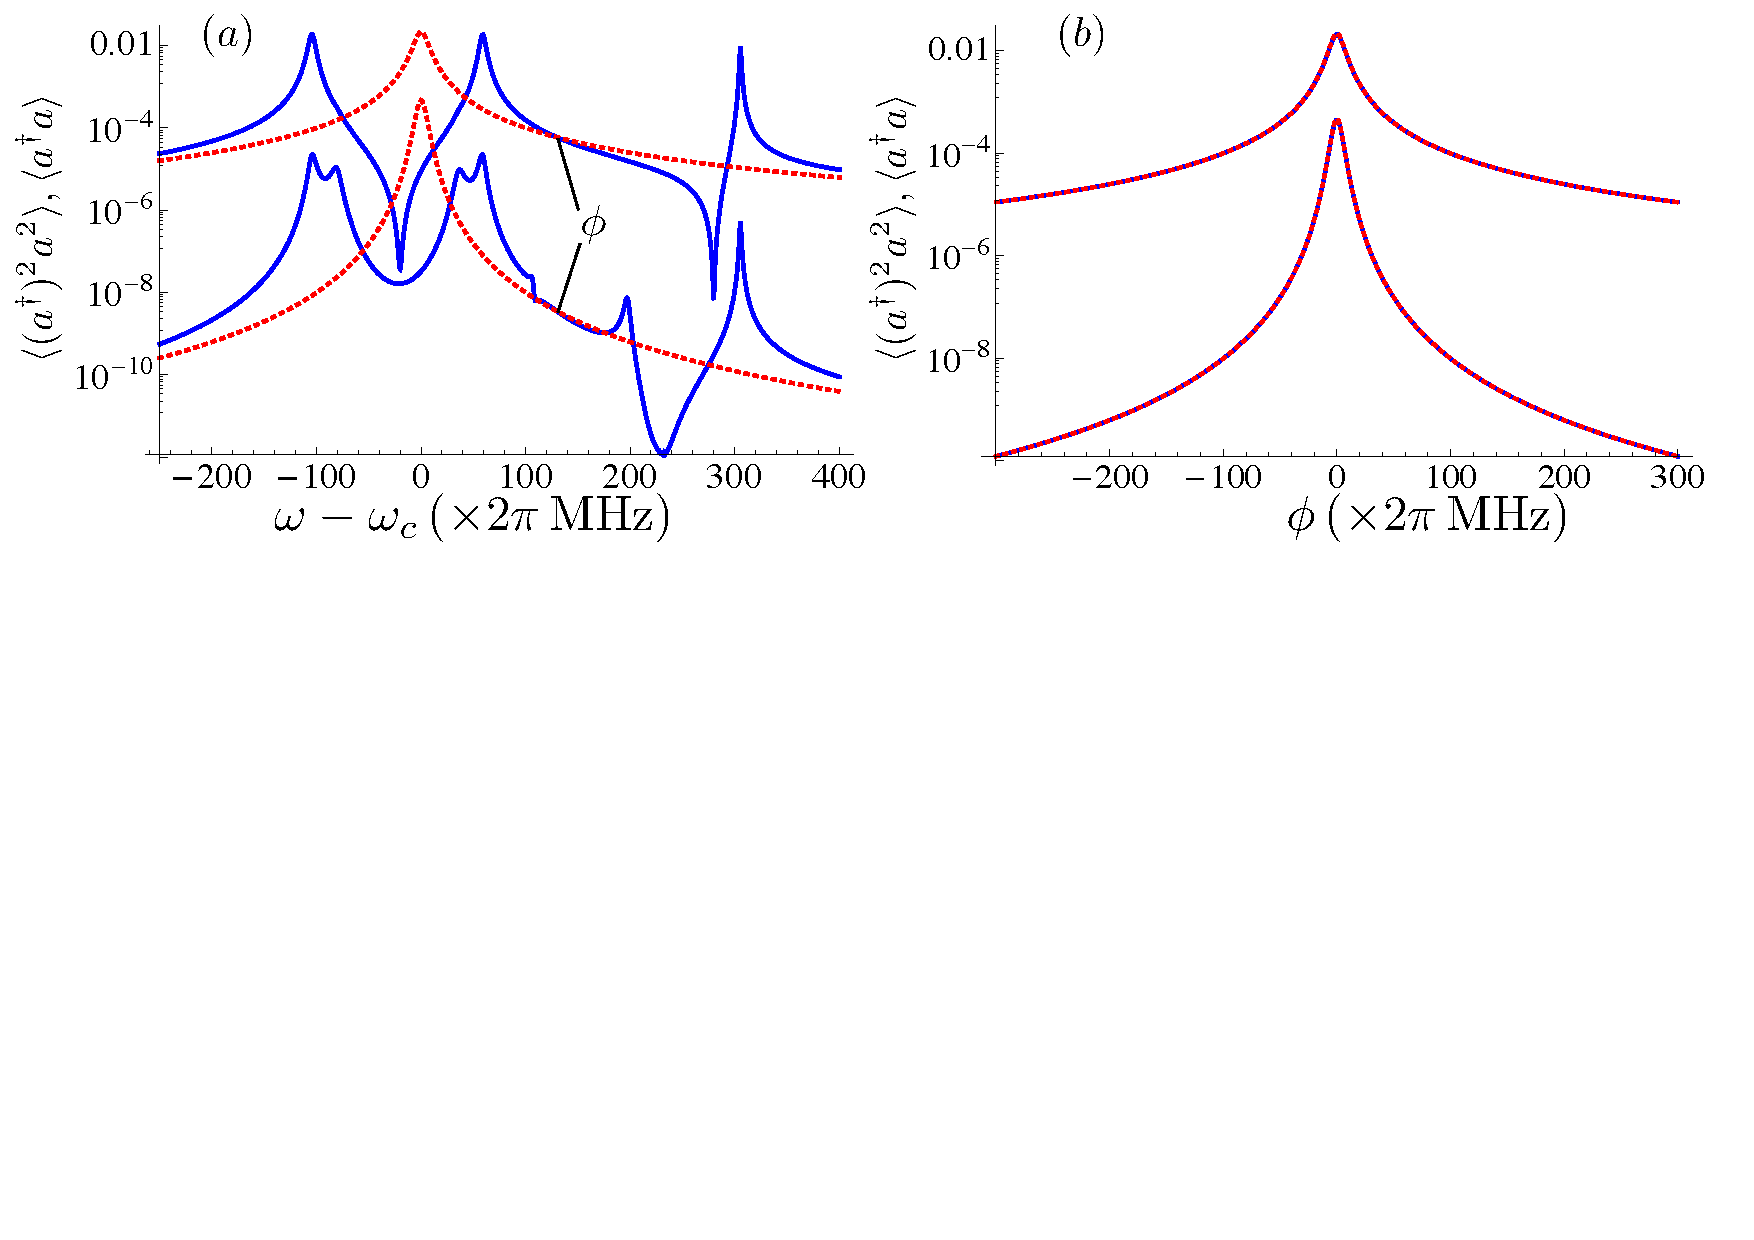
\includegraphics[width=\textwidth]{Images/chap5/transparency.pdf}
    \caption[ $\langle a^\dagger a \rangle$ and $\langle (a^\dagger)^2 a^2 \rangle$ in function of $\omega-\omega_c$ ]{On $(a)$, spectra of $\langle a^\dagger a \rangle$ (top) and $\langle (a^\dagger)^2 a^2 \rangle$ (bottom) in function of $\omega-\omega_c$ for the values in Tab.~\ref{tab-values}, $\epsilon= 2\pi\,\mbox{MHz}$, $\Delta=150\times 2\pi\,\mbox{MHz}$ and $\phi=130\times 2\pi\,\mbox{MHz}$ (blue) along with the same spectra of an empty cavity (red, dotted) with the same settings and $\alpha=0$. On $(b)$, the same spectra of the system with the laser frequency set on $\omega = \omega_c + \phi = (\omega_1+\omega_2)/2$  in function of $\phi$ (blue), along with the spectra of the empty cavity (red, dotted). At the frequency $2\omega= \omega_1+\omega_2$, the system behaves as if the atoms were not in the cavity. }
    \label{fig-transparency}
\end{figure}

We showed in Fig.~\ref{fig-transparency} $(a)$ the same plot as in Fig.~\ref{fig-aa_cool_150} (blue) along with the spectrum obtained by setting the atom-field coupling constant $\alpha$ to zero (red, dotted). We noted that at the frequency $\omega= (\omega_1+\omega_2)/2=\omega_c+\phi$ both red lines crossed the blue lines. In other words, at that particular frequency, the number of photons in the cavity is exactly the number of photons that would be expected in an empty cavity, furthermore the same result holds for the mean number of pairs of photons. It is easy to check numerically that the relation
\[\mean{(a^\dagger)^2 a^2}=(\mean{a^\dagger a})^2,\]
also holds for our two-atom system at the frequency $2\omega= \omega_1+\omega_2$.

In Fig.~\ref{fig-transparency} $(b)$ we plotted $\mean{a^\dagger a}$ and $\mean{(a^\dagger)^2 a^2}$ in function of $\phi$ for a laser frequency $\omega = \omega_c + \phi = (\omega_1+\omega_2)/2$ (blue) along with the same quantities obtained for an empty cavity (red, dotted) for comparison. The two plots are identical, signature of some kind of cavity induced transparency (CIT) of the system.

Those figures were plotted with the atomic frequency difference $\Delta=150\times 2\pi\,\mbox{MHz}$, however we may recall that the all the photon spectra we presented showed dips at the atomic frequencies $\omega_1$ and $\omega_2$ (although not very obvious on Fig.~\ref{fig-spec150} due to the large value of $\epsilon$), we would therefore suspect that the transparency effect would not be observed  when the atoms have identical frequencies, i.~e.~when $\Delta=0$. Indeed, the mean number of photons in a cavity with a laser on resonance with two identical atoms does not go beyond $\mean{a^\dagger a} \simeq 3 \; 10^{-10}$, a value of about 6 orders of magnitude smaller than the one obtained for $\Delta=150\times 2\pi\,\mbox{MHz}$.

\begin{figure}
    \center
    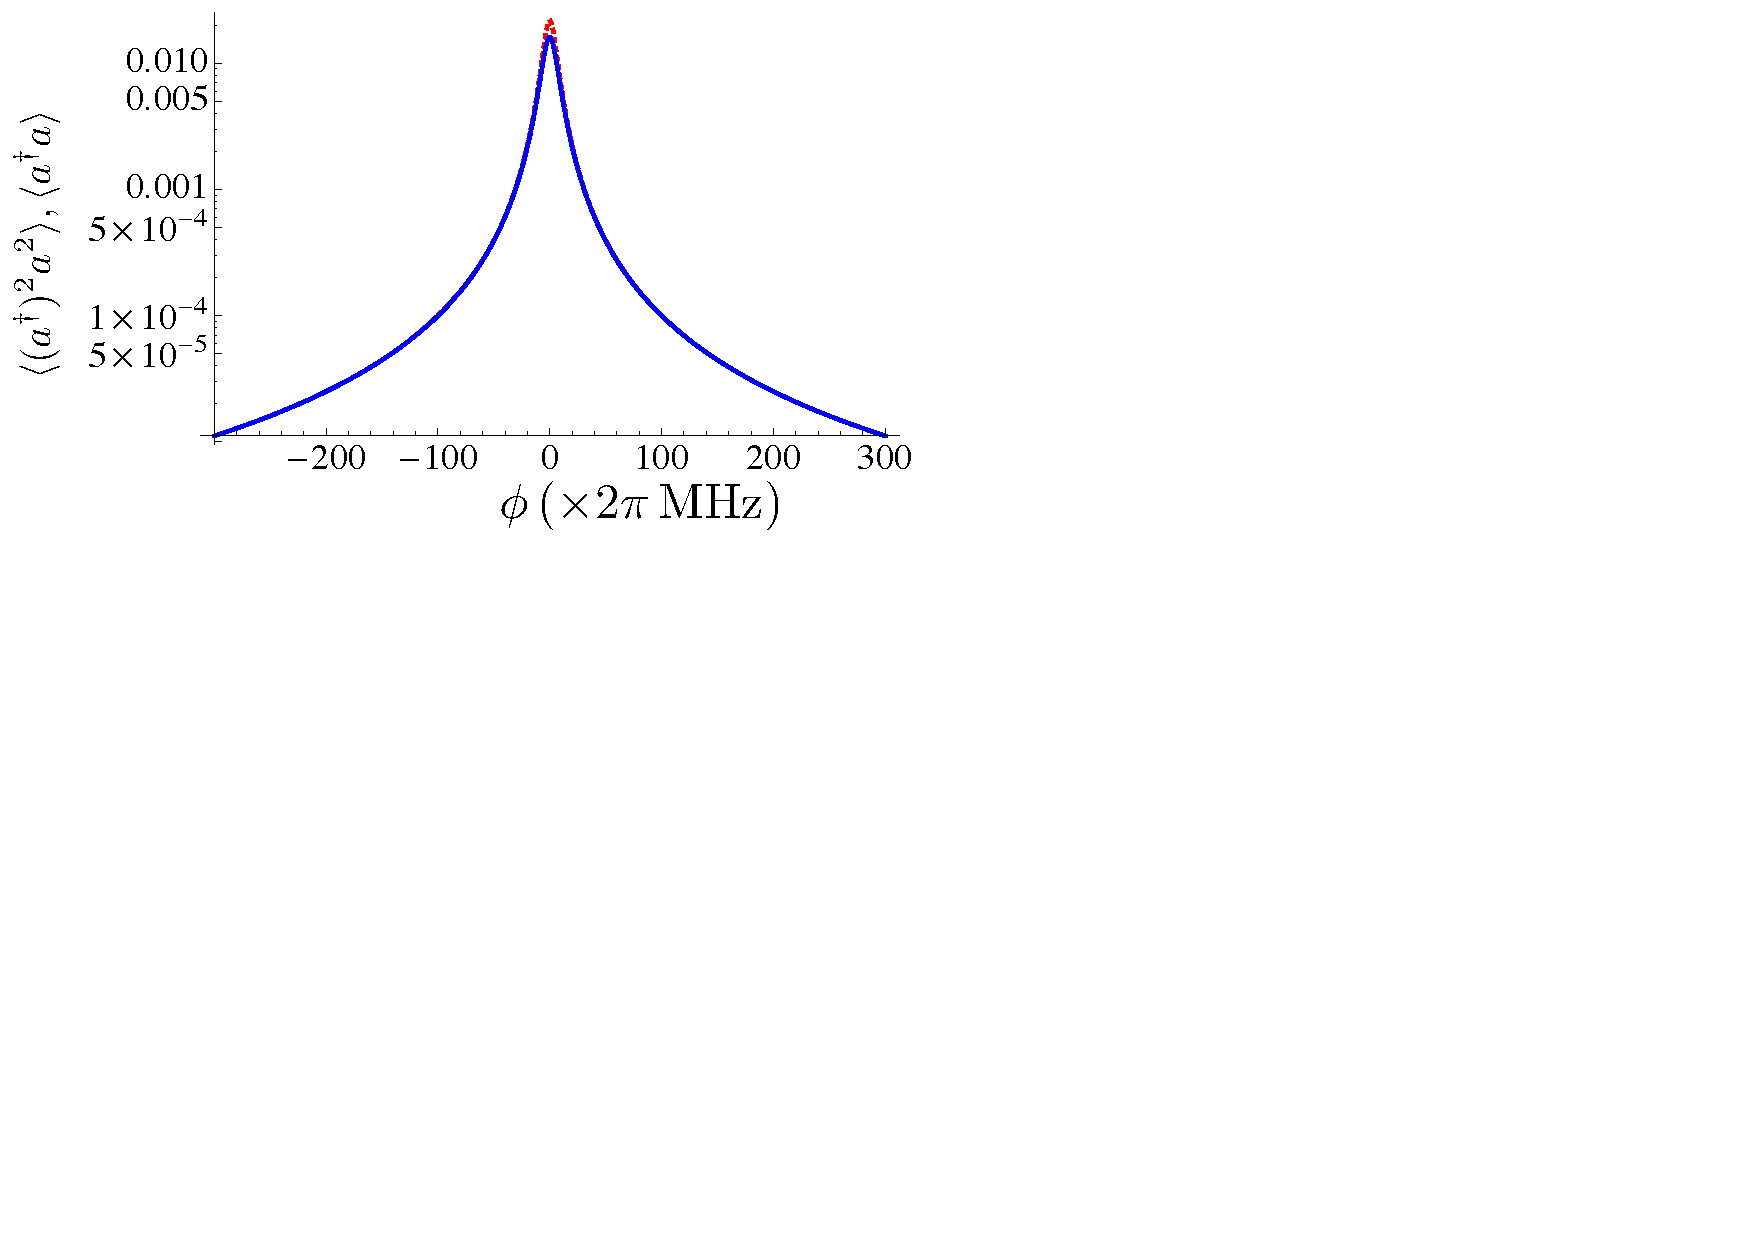
\includegraphics[width=0.65 \textwidth]{Images/chap5/transparency50.pdf}
    \caption[$\langle a^\dagger a \rangle$  and $\langle (a^\dagger)^2 a^2 \rangle$ ]{Spectra of $\langle a^\dagger a \rangle$ (top) and $\langle (a^\dagger)^2 a^2 \rangle$ (bottom) of the system with the laser frequency set on $\omega = \omega_c + \phi = (\omega_1+\omega_2)/2$ in function of $\phi$ (blue) along with the spectra of the empty cavity (red, dotted). The CIT effect is not perfectly observed around $\phi=0$ since the atom frequencies are not spread out enough.}
    \label{fig-transparency50}
\end{figure}

In Fig.~\ref{fig-transparency50} we plotted the same plot as in Fig.~\ref{fig-transparency} $(b)$, but with a smaller gap in atomic frequencies $\Delta =50 \times 2\pi\,\mbox{MHz}$. We can see that on most of the spectrum the CIT effect is observed, although around $\phi=0$ the number of photons in the cavity is slightly smaller than what it would be in an empty cavity. We conclude that the CIT effect is stronger when the gap in the atomic frequencies is larger and not in competition with the cavity decay induced photon inhibition at the atomic frequencies.

We see on Fig.~\ref{fig-trans} that the $(\omega_1+\omega_2)/2$ values for non-zero $\phi$ never coincide with another transition value, therefore we should not expect a strong competition between the CIT and other transition resonances.

\section{Summary and Discussion} \label{sec-QEDconcl}

In this chapter, we have studied the behavior of two unidentical two-level atoms in a single mode cavity driven by a laser under realistic conditions of spontaneous emission and cavity losses. In free space, two-photon processes for independent atoms do not happen, as we checked by using perturbation theory and further with a master equation calculation. Our next objective was to show that two-level processes are possible in a cavity ad to study their occurrences in realistic experimental conditions.

In order to study the system using perturbation theory, we made the simplification of considering two atoms with frequencies evenly spread around the cavity mode frequency. We were then able to express analytically the eigenstates and eigenvalues of the unperturbed Hamiltonian, which allowed us to show that two-photon processes were possible for different dressed states of the system. In the free space case, the two-photon processes would have to happen at the mean of the atomic frequencies, but we found that in a cavity the transitions at that particular frequency were merely one-photon processes which could however be suppressed if the two atoms were identical with internal frequencies equal to the cavity's.

We confirmed that analysis with the steady states of the master equation and we observed peaks due to multi-photon processes, up to five-photon processes in a perfect cavity\footnote{Five-photon processes are obviously the highest multi-photon processes one could obtain with a truncated basis with $n_{\mbox{max}}=5$. However, attempts were made with $n_{\mbox{max}}=7$ and no higher order process was noticed for the same value of $\epsilon$.}. The mean number of photons in the cavity, the mean number of pairs of photons, the population of a single excited atom as well as the population of two excited atoms in the system were studied.

Some effect that were not expected from the perturbation theory were observed for important cavity decay rates. Dips in the mean number of photons spectra were found whenever the laser hit the atomic frequencies. The population of two excited atoms was strongly weakened when the laser frequency was in the middle of the atomic frequencies but peaked on the atomic frequencies themselves for very poor quality cavities. Also for those cavities,  the population of a single excited atom peaked when the laser resonated with its frequency but dipped for the other atom's frequency. The shifting of the peaks is understood easily as when the cavity loses more and more photons, it becomes similar with free space. However some kind of coupling still remains and causes dips that are not observed in free space.

The purely numerical study of steady states of the system without the simplification on the atomic frequencies was also conducted. The degeneracies on some dressed states were lifted and the number of one and two-photon peaks augmented as could have been expected. The results coming from the cavity decay processes were also observed and confirmed to exist in the general case.

A last effect, the cavity induced transparency, was observed. We showed that when the laser frequency was in the middle of the atomic frequencies, not only the population of the doubly excited state dropped but also the number of photons and of pairs of photons were found to be identical to the number that would have been found in an empty cavity, therefore yielding no particular multi-photon process, exactly as what we found in free space. The CIT effect was not found to be as strong when the atomic frequencies were very close from each other, as in this case the cavity decay induced drop in the mean photon number takes precedence.

Actual experimental realizations of atoms in resonant cavities have been realized in circuit cavity QED. In that type of experiments, like in~\cite{Fin08, Fin09,Bau09} a lot of parameters, such at the atomic frequencies, are independently controllable. Monitoring the transmission at low enough power exhibits the usual vacuum Rabi splitting, specific to two atoms as the Rabi splitting depends on the number of atoms~\cite{San83, Aga84, Rai89, Boc04, Mau05, tho98}. With an increase of the input power, the transmission could show the cavity two-photon resonance and exhibit all the effects we spoke of. A particular immediate realization of that two-photon effect could be realized in circuit cavity QED considering the setup used in~\cite{Fin09} with two superconducting qubits instead of three. In that experiment, the frequency of each qubit is separately tunable, and we deliberately chose in this paper parameters close to what has been achieved.

Clearly, the existence of cavity induced two-photon transition implies the existence of cavity induced inter-qubits interaction. This would suggest that all inter-atomic forces can be manipulated by using cavities, as we have control over parameters like frequencies or coupling strengths. Cavities offer many possibilities, as whole ladders of dressed states and one or more external fields can be used to manipulate interactions inside the cavity~\cite{sol03, Bir05}.

 

%----------------------------------------------------------------------------------------
%	BIBLIOGRAPHY
%----------------------------------------------------------------------------------------

\addtocontents{toc}{\vspace{2em}} % Add a gap in the Contents, for aesthetics
\unnumberedchapter{Bibliography} % Title of the unnumbered chapter
\bibliography{Preamble/Thesis_bibliography} % The references information are stored in the file named "Thesis_bibliography.bib"

%----------------------------------------------------------------------------------------
%	APPENDICES
%----------------------------------------------------------------------------------------

\addtocontents{toc}{\vspace{2em}} % Add a gap in the Contents, for aesthetics
\appendix % Starts of appendices

\numberedchapter


\chapter{Appendices} \label{appA}

Please refer to \url{https://groups.oist.jp/grad/academic-program-policies} for specifications.

%\input{MainText/appendixB}
%\input{MainText/appendixC}

\end{document}  
